% !TeX encoding = UTF-8
% !TeX spellcheck = en_US

%*******************************************************************************
%* Work Configuration
%*******************************************************************************
\title{An Ontology of Student Consulting Organizations}
\author{Felix Förtsch}
\documentclass[a4paper, DIV=13, BCOR=0cm]{scrbook}

%*******************************************************************************
%* Packages
%*******************************************************************************
\usepackage[english]{babel}
\usepackage[
	backend=biber,
	style=numeric,
	urldate=iso,
	sorting=none
	]{biblatex}
\usepackage{xcolor} % Für Farben im Text
\usepackage{xstring} % String-Manipulation; wird von anderen Paketen oft verwendet
\usepackage{fontspec} % Einstellungen für Schriftarten (zB lokales Laden)
\usepackage{csquotes} % Verwaltet Anführungsstriche
\usepackage[hidelinks]{hyperref} % Hyperlink-Helfer
\usepackage[defblank]{paralist} % Erlaubt verschiedene neue Listen-Umgebungen (zB inparaenum), defblank für Listenumgebung, die gesetzt wird wie regulärer Text
\usepackage{mdframed} % Erlaubt das einfügen von Kästen (zB Einrahmen von Anmerkungen)
%\usepackage{lscape} % Querformat-Umgebung
\usepackage[toc, section=section, numberedsection=autolabel, nonumberlist]{glossaries} % Glossar
\usepackage[titletoc]{appendix}
\usepackage{progressbar}
\usepackage{tikz}
\usepackage{multicol} % Mehrfachspalten-Umgebung

%*******************************************************************************
%* Configuration
%*******************************************************************************
% Language
\selectlanguage{english}

% Bibliography
\bibliography{main}
\KOMAoptions{bibliography=numbered}
\KOMAoptions{bibliography=leveldown}

% Table of Contents
%\setcounter{tocdepth}{\paragraphtocdepth}

% SubSubsection numbering
%\setcounter{secnumdepth}{5}

% Layout Settings
\KOMAoptions{draft=false}
\KOMAoptions{twoside=false}
\KOMAoptions{titlepage=true}
%\KOMAoptions{headings=small}
\KOMAoptions{parskip=half} % Deaktiviert den den Absatzeinzug

% Header and Footer
\pagestyle{myheadings}
\KOMAoptions{headsepline=true} % Aktiviert eine Trennlinie zwischen Header und Dokument
%\KOMAoptions{footnotes=multiple}

% Style
%\setmainfont[
%	Path=Fonts/,
%	Extension=.ttf,
%	UprightFont=*,
%	BoldFont=*-Bold,
%	ItalicFont=*-Italic,
%	BoldItalicFont=*-BoldItalic
%]{DejaVuSerif}
%\setmonofont[
%	Path=Fonts/,
%	Extension=.otf,
%	UprightFont=*-Regular,
%	BoldFont=*-Bold,
%]{FiraCode}

% mdframed Styles
\global\mdfdefinestyle{onto}{%
	linewidth=1pt,%
	frametitlerule=true,%
	frametitlerulecolor=black,%
	frametitlerulewidth=2pt,%
	frametitlebackgroundcolor=gray!20,%
	frametitlefont=\textbf%
}

\global\mdfdefinestyle{onto-1}{%
	leftmargin=20pt,
	linewidth=1pt,%
	frametitlerule=true,%
	frametitlerulecolor=green,%
	frametitlerulewidth=2pt,%
	frametitlebackgroundcolor=gray!20,%
	frametitlefont=\textbf%
}

\global\mdfdefinestyle{onto-2}{%
	leftmargin=40pt,
	linewidth=1pt,%
	frametitlerule=true,%
	frametitlerulecolor=blue,%
	frametitlerulewidth=2pt,%
	frametitlebackgroundcolor=gray!20,%
	frametitlefont=\textbf%
}

\global\mdfdefinestyle{onto-3}{%
	leftmargin=60pt,
	linewidth=1pt,%
	frametitlerule=true,%
	frametitlerulecolor=orange,%
	frametitlerulewidth=2pt,%
	frametitlebackgroundcolor=gray!20,%
	frametitlefont=\textbf%
}

\global\mdfdefinestyle{onto-4}{%
	leftmargin=80pt,
	linewidth=1pt,%
	frametitlerule=true,%
	frametitlerulecolor=red,%
	frametitlerulewidth=2pt,%
	frametitlebackgroundcolor=gray!20,%
	frametitlefont=\textbf%
}

\global\mdfdefinestyle{dictionary}{%
	linewidth=1pt,%
	frametitlerule=true,%
	frametitlebackgroundcolor=gray!20,%
	innertopmargin=\topskip,%
	frametitlefont=\textbf%
}

%*******************************************************************************
%* Macros
%*******************************************************************************
\newcommand{\eg}{e.\,g.\ }
\newcommand{\Eg}{E.\,g.\ }
\newcommand{\aka}{a.\,k.\,a.\ }
\newcommand{\class}[1]{\texttt{\textbf{#1}}}
\newcommand{\relation}[1]{\texttt{#1}}
\newcommand{\prop}[1]{\texttt{#1}}
\newcommand{\pn}[1]{\textit{\textbf{#1}}}
\newcommand{\foottt}[1]{\footnote{\texttt{#1}}}
\newcommand{\link}[2]{\href{#1}{$\hookrightarrow$#2}}

%*******************************************************************************
%* Glossar
%*******************************************************************************
\glsdisablehyper % Disables hyperlinks for the glossary
\makenoidxglossaries

% Acronyms
\newacronym{sco}{SCO}{Student Consulting Organization}
\newacronym{je}{JE}{Junior Enterprise}
\newacronym{bdsu}{BDSU}{\link{https://bdsu.de}{Bundesverband Deutscher Studentischer Unternehmensberatungen}}
\newacronym{jcn}{JCNetwork}{\link{https://jcnetwork.de}{Junior Consultant Network}}
\newacronym{hc}{HC}{\link{https://hanseaticconsulting.de}{Hanseatic Consulting}}
\newacronym{ci}{CI}{\link{https://campusinform.de}{Campus Inform}}
\newacronym{kiss}{KISS}{Keep It Stupid Simple}
\newacronym{aktg}{AktG}{Aktiengesetz}
\newacronym{gmbhg}{GmbHG}{Gesetz betreffend die Gesellschaften mit beschränkter Haftung}
\newacronym{foaf}{FOAF}{Friend of a Friend}
\newacronym{dcmi}{DCMI}{Dublin Core Metadata Initiative}
\newacronym{dcmt}{DCMT}{Dublin Core Metadata Terms}
\newacronym{bfo}{BFO}{Basic Formal Ontology}
\newacronym{gfo}{GFO}{General Formal Ontology}
\newacronym{fibo}{FIBO}{Financial Industry Business Ontology}
\newacronym{gist}{GIST}{GIST}
\newacronym{schema}{Schema.org}{Schema.org Ontology}
\newacronym{doap}{DOAP}{Description of a Project}
\newacronym{bpmn}{BPMN}{Business Process Modeling and Notation}
\newacronym{bpmno}{BPMNO}{Business Process Modeling and Notation Ontology}
\newacronym{epc}{EPC}{Event-Driven Process Chain}
\newacronym{uml}{UML}{Unified Modeling Language}
\newacronym{psl}{PSL}{Process Specification Language}
\newacronym{nist}{NIST}{National Institute of Standards and Technology}
\newacronym{opm}{OPM}{Object Process Methodology}
\newacronym{hrp}{HRP}{Human Resource Process}
\newacronym{pp}{PP}{Project Process}
\newacronym{oc}{OC}{Organizational Context}
\newacronym{pc}{PC}{Project Context}
\newacronym{co}{CO}{Corporate Officer}
\newacronym{ceo}{CEO}{Chief Executive Officer}
\newacronym{cfo}{CFO}{Chief Financial Officer}
\newacronym{cto}{CTO}{Chief Technical Officer}
\newacronym{clo}{CLO}{Chief Legal Officer}
\newacronym{coo}{COO}{Chief Operating Officer}
\newacronym{iso}{ISO}{International Organization for Standardization}
\newacronym{pm}{PM}{Project Management}
\newacronym{owl}{OWL}{Web Ontology Language}
\newacronym{w3c}{W3C}{World Wide Web Consortium}
\newacronym{rdf}{RDF}{Resource Description Framework}
\newacronym{rdfs}{RDFS}{Resource Description Framework Schema}
\newacronym{skos}{SKOS}{Simple Knowledge Organization System}
\newacronym{eo}{EO}{Enterprise Ontology}
\newacronym{iri}{IRI}{Internationalized Resource Identifier}

% Special Plurals
\newglossaryentry{tlo}{name={TLO}, description={Top-Level Ontology}, descriptionplural={Top-Level Ontologies}, firstplural={\glsentrydescplural{tlo} (\glsentryplural{tlo}, also sometimes called \textit{Upper Ontologies})}}
\newglossaryentry{udo}{name={UDO}, description={Upper-Domain Ontology}, descriptionplural={Upper-Domain Ontologies}, firstplural={\glsentrydescplural{udo} (\glsentryplural{udo})}}
\newglossaryentry{do}{name={DO}, description={Domain Ontology}, descriptionplural={Domain Ontologies}, firstplural={\glsentrydescplural{do} (\glsentryplural{do})}}


%*******************************************************************************
%* Dokumentenanfang
%*******************************************************************************
\begin{document}

\titlehead{
	Document Version: v22 \\
	Overall Progress: \progressbar[filledcolor=green]{0.99}
}
\subject{Bachelor's Thesis}
\title{Student Consulting Organizations}
\subtitle{A Domain Ontology}
\author{Felix Förtsch \\ 3708438 }
\date{13.07.2020}
\publishers{Leipzig University \vspace{1cm} \\
	Supervised by: \\
	Prof. Dr. Heinrich Herre \\
	Dr. Frank Loebe \vspace{0.5cm}}
\maketitle

\frontmatter
\chapter*{Abstract}
	This work develops a domain ontology for Student Consulting Organizations. The model declares the domain knowledge and defines its vocabulary. It is a primer to be a starting point to establish or run such an organization in a university context. Additionally it allows for optimization in existing organizations and contributes to cooperation between SCO by organizing existing knowledge. It maximizes the use of vocabularies, relations, and classes from established ontologies to link the domain knowledge into a bigger context. The main resource of the developed ontology are SCOs from Germany, but the concepts can be transferred and made applicable in a wider area.
	
	The primary classes of the domain are: \class{Agent}, \class{Document}, \class{Process}, \class{Project}, and \class{Role}. At the core of the domain are processes and projects, while agents are their actors playing certain roles. The core processes are the \class{Project Process} and the \class{Human Resource Process}.
	
	%TODO: Add numbers (how many classes, axioms etc)

\chapter*{Formatting}
\begin{itemize}
	\item Hyperlinks are embedded and clickable in the PDF. They are marked with an arrow and a light blue border: \link{https://hyperlink.com}{Hyperlink}
	\item Everything related to the ontology implementation, such as references to classes or relations, is written as \texttt{typewriter text}.
	\item Relations are written in camelCase: \texttt{subclassOf}
	\item Classes are bold, capitalized, and use Snake\_Case: \texttt{\textbf{Awesome\_Class}}
	\item Name spaces may be added to a class for clarification; they are separated by a colon: \class{namespace:Class}
	\item Citations directly behind a statement apply to only this statement. Citations after a full stop apply to the whole sentence.
	\item Citations are clickable in the PDF and forward directly to the bibliography.
	\item The bibliography is sorted by order of appearance.
\end{itemize}

%\chapter*{}
%\newpage

\tableofcontents
\newpage

\mainmatter
\chapter{Introduction}
\markright{1. Introduction}
\section{Motivation}
\glspl{sco}\footnote{Also known as 
\link{https://en.wikipedia.org/wiki/Junior_enterprise}{Junior Enterprises} in some parts of the world.} are student-run consulting businesses that focus on teaching their members essential business and life skills exceeding the theoretical knowledge from university. They are very similar to small to medium consulting businesses, but are run and organized---most of the time exclusively---by students. Even though the concept is not universally known, this kind of organization exists worldwide and has a history dating back to at least 1967\footnote{The founding of \link{https://www.en.junioressec.com/}{Junior ESSEC} in the context of the ESSEC Business School in France.}. Germany has two different umbrella organizations for \glspl{sco} that together have more than 60 member organizations.\footnote{\gls{bdsu}, \gls{jcn}}

But as far as we know, there has not yet been any effort to collect and compose the existing domain knowledge of German \glspl{sco} in a publicly available and usable form. We consider this an important task, since it is a contribution to prevent knowledge loss that is inherent in the dynamics of these organizations: the majority of the staff are students and thus their consulting career is inherently linked to their university career:

\begin{enumerate}
	\item The career is time-bound to the duration of the education. A bachelor's degree in Germany averages 7,5-7,6 semesters and a master's degree 4,2-4,5 semesters, which adds up to a total of 11,7-12,1 semesters or ca. six years. \cite{stabu2019a} This frames the available time for the transfer of the domain knowledge.\footnote{There sometimes are also PhD students, but they can be considered outliers and are atypical.}
	\item The career is parallel to the curriculum. From our experience, freshmen that decide to join student organizations typically do so at the beginning of their second or third semester, after they got acclimated with the workload of their university classes. Since students usually participate in parallel to their education---and the focus is typically on the education\mbox{---,} they have to manage their time accordingly, which reduces time spent with the \gls{sco}. Furthermore, students may have other (\eg personal) interests that compete with the same time budget.
\end{enumerate}

The reasons above reduce the available time for knowledge transfer and persistence and make these problems harder. Many \glspl{sco} have worked on and developed solutions to help with this problem. Some of them are informal, some formal in nature. For example: One particular organization we worked with, \gls{hc}, used process methodology to document much of their knowledge. Another one we worked with, \gls{ci}, focused on lectures and training sessions.

However, the majority of available domain documents are highly individualized and miss the necessary level of abstraction to make them directly applicable to other \glspl{sco}. But even though every \gls{sco} is organized slightly differently from the next, uses different vocabulary and each has their individual culture, they all share the idea of teaching consulting and project work to their members. Since they aim for the same goal, they are very similar at their core.

Therefore we try to contribute a more general model in the form of an ontology that tries to combine the domain knowledge, vocabulary, and common concepts.

\section{Goal and Scope of the Work}
\label{goal}
\paragraph{Goal}
The goal of this work is the description of one abstract \gls{sco}. It extracts the available implicit expert knowledge, links it with related work, and transforms it into explicit  knowledge by presenting it as an ontology. It defines common classes and relations required to describe such an organization using domain vocabulary. Additionally it provides terminology explanations, background knowledge, and links into other ontologies where it is sensible.

\paragraph{Deliverables}
\begin{quote}
	\enquote{A deliverable is a tangible or intangible good or service produced as a result of a project that is intended to be delivered to a customer.} \cite{deliverable}
\end{quote}

The deliverable output of this work are two documents:
\begin{enumerate}
	\item This thesis as a documentation and explanation of the ontology development process including but not limited to: methodology, background information, decisions in regarding the ontology, etc.
	\item The ontology document as a representation of the domain knowledge in the \gls{owl}.
\end{enumerate}

Both documents will be publicly hosted and freely available to any interested parties, such as umbrella organizations, \glspl{sco}, or students.
%TODO: Host the document publicly

\paragraph{Out of Scope}
\begin{itemize}
	\item This work is not a thesaurus or dictionary.
	\item This work is not a documentation about a \textit{specific} \gls{sco}.
	\item This work does claim to provide a \textit{complete} model for the domain. It models the domain to the best of the authors ability provided the context, time, and manpower.
	\item This work will not deliver an example instance.
	\item The ontology will not include the individual project process, since projects differ vastly between each other and more general ontologies and frameworks for projects already exist.
	\item Furthermore it will not model projects further than declaring them. As already stated above, there are many project (management) concepts available.
\end{itemize}

\section{Use Cases and Outlook}
The main use case of this work is supporting \gls{sco} idea by the documenting the domain knowledge and thus helping others to better understand it. We are trying to design the ontology in a way to enable its use for everyone: From the layperson to the expert.

We identified the following additional use cases from our personal experience and hope that this work can contribute to them in a meaningful way:

\begin{enumerate}
	\item \textbf{Founding of a \gls{sco}.} Founding an business is hard. It becomes even more challenging, if there are no available learning materials for the domain, the learning materials are hidden away, or the materials offer low quality. And even though many of the \glspl{sco} in Germany have produced a lot of material and each figured out their own way of doing things, and even though there are umbrella organizations to help organize all the sub-organizations, it is still hard for the target audience to get sufficient information to easily found such an organization. This work can support this process by providing basic insight into the inner workings the domain. It sheds light on its most important processes and actors. It can provide the new founders with knowledge and a guideline on what to focus on. The public availability further supports this idea.
	\item \textbf{Optimization.} Many \gls{sco} are already adapt at looking critically at their workflows and getting better at what they do. But there is always room for improvement. Process analysis and management are tools to contribute to this path of optimization. This works provides the fundamental perspective on this topic and focuses on the two core processes that have to be dealt with in the \gls{sco} context: The Project Process and the Human Resources Process. Furthermore, other structural elements (\eg leadership elementary roles) are provided. Any \gls{sco} can use this work as an anchor for comparison.
	\item \textbf{Backbone for Domain Specific Software Projects.} This work provides a high-level conceptual model of the \gls{sco} domain. Furthermore, it provides concept descriptions and context while being computer-readable. Hence, this work can be used as a backbone and starting point for software projects that want to target the domain.
\end{enumerate}

\chapter[Preliminaries \\\textcolor{gray}{
	{\footnotesize \textsl{Gives the background of this work and prepares for the subsequent elucidation.}}
}]{Preliminaries}
\markright{2. Preliminaries}
Ontologies have many applications in various fields. They are used in artificial intelligence research, database design and integration, semantic web, and many more. \cite[p.\,1]{Gomez-Perez:2004aa} One of these applications is knowledge representation.

\begin{quote}
	\enquote{\textbf{Knowledge Representation} is the field of Artificial Intelligence that focuses on the design of formalisms that are both epistemologically and computationally adequate for expressing knowledge about a particular domain.} \cite[p.\,XV, Preface]{baader2017introduction}
\end{quote}

This work is concerned with the knowledge representation of one particular domain: \glspl{sco}. The following section describes how we approach the development of this particular ontology, define the necessary vocabulary and relations between the terms, and explore the domain structurally.

\section{Methodology for the Development of the Ontology}
\label{methodology}
The primary goal of this work (see \autoref{goal}) is the creation of a particular domain ontology. Our language of choice for this task is \gls{owl}. It is an ontology language developed by the consensus-driven and well respected \gls{w3c}. \cite[p.\,206]{baader2017introduction} It is widely used and offers very good tooling in the ontology editor \link{https://protege.stanford.edu}{\pn{Protégé}}, which is built and maintained by ontology researchers of \pn{Stanford University}. \cite{musen2015protege} Furthermore the research group provides an ontology development methodology \cite{guide-to-ontology} that we can build upon. It involves the following steps:
\begin{compactenum}
	\item Determine the domain and scope of the ontology,
	\item consider reusing existing ontologies,
	\item enumerate important terms in the ontology,
	\item define the classes and the class hierarchy,
	\item define the properties of classes-slots\footnote{The guide is written for an earlier version of Protégé and the terms have since been updated. Slots are now referred to as annotations and facets are the data types of annotations.},
	\item define the facets of the slots\footnote{See above.}, and
	\item create instances.
\end{compactenum}

It is important to note that even though these steps look like they should be performed sequentially, this is not the case. Instead, the ontology starts out as a draft and is refined during development \cite[Section 3, Introduction]{guide-to-ontology}, following the iterative approach, that is common for ontology development. \cite[p.\,158, section 1.5.1]{stuckenschmidt2010ontologien} This quickly becomes apparent during the process of answering the suggested \pn{Competency Questions} to (1) determine the domain and scope of the ontology \cite[Section 3, Step 1]{guide-to-ontology} and taking into account (2) existing ontologies. And this also is true for steps (3) to (6). Therefore the steps are grouped together to make the overall structure of this work easier to follow.

The phases of the methodology are discussed in more detail in the following two sections and group the proposed steps as follows:

\begin{compactenum}
	\item Steps 1 and 2 are performed during the \pn{Research Phase}.
	\item Steps 3 to 6 during the \pn{Analysis and Synthesis Phase}.
\end{compactenum}

The last step, (7) the creation of instances, is omitted in this work. It is only really relevant if the ontology is used to describe one specific \gls{sco}. However, this ontology is operating on a higher level of abstraction, trying to describe a more general case.

%TODO: Onto-Axiomatische Methode von Herrn Herder Abschnitt 2

\subsection{Research Phase}
To our understanding, the main goal of the first part of the methodology is the creation of a foundation for the ontology: It needs to have a clearly defined scope. Additionally the recommended reuse of other ontologies helps creating a web of linked knowledge and reduces the amount of duplicate work.

To find a starting point for data collection and identify existing ontologies, we take an intuitive first look at \glspl{sco} and their driving factor:

\begin{mdframed}
	\textbf{The Idea of Student Consulting Organizations}\\
	Selecting a career is a very difficult and important choice in a young persons life. University education is closely linked to this choice and entering a specific field often requires a specific degree (\eg to become a lawyer, a student has to pass the bar exam).

	Most universities know this and have set up dedicated offices to offer career advice to their students. They not only help picking a fitting course of studies at the beginning of a university career, but also help the students to aim for a fitting job.

	Doing an internship with a company working in the field the student is interested in, is a widespread recommendation. It allows for a glimpse into the profession as well as gathering work experience.

	\glspl{sco} offer an option to investigate a career in business consulting, as well as learning the associated skills and getting paid in the process. They offer the students a way to learn about concept like project based work---the modus operandi of consulting companies---, \eg project planning and management, as well as structuring and presentation of information.

	Consulting is a very diverse field of work. Since consulting can be applied to any field of business, it can be used as a stepping stone into a career.
\end{mdframed}

Observing this intuitive perspective, we can see, that \glspl{sco} are connected to other knowledge domains in various ways: They are a type of social organization and thus are driven by people and processes. Organizations and in extension their processes have actors with responsibilities. This is a hint that the concept of roles might be a part of the ontology. \glspl{sco} can be generally considered a form of business and therefore business aspects have to be taken into account. The fact that they do consulting work creates a connection into the domain of (business) consulting and the domain of projects, since consulting work is project based.

This intuitive approach generates a starting point for the research:
\begin{itemize}
	\item Previously developed ontologies in related domains, \eg consulting, project management, educational organizations.
	\item Available domain knowledge, \eg process documentation of \gls{hc} and \gls{ci}.
	\item Personal expert domain knowledge and peer-review by other \gls{sco} members.
\end{itemize}

Furthermore it implies some more general research topics such as the implications of other general, upper-domain, and top-level ontologies as well as theory of description logic and theory of ontologies (\eg modeling of roles and processes).

Defining the scope of the ontology is the formal step that concludes the \textit{Research Phase}. This work accomplishes this by answering the Competency Questions. Since the questions can be considered a part of the ontology, they and their corresponding answers can be found as part of the ontology in \autoref{competency-questions}.

\subsection{Analysis and Synthesis Phase}
\label{analysis}
The majority of this work happened during the Analysis and Synthesis Phase. Its goal is the review, interpretation, and structuring of the collected data; ultimately generating an ontology in the target format \gls{owl}.

Based on the Protégé-methodology, the first two steps of this phase are: (3) the creation of an enumeration of terms that are relevant for the domain. And (4) the translation of the terms into the backbone of every ontology: the class hierarchy. Both are rooted in the results of the previous phase and further supplemented by expert knowledge.

At the core of this thought process is the conversion of available implicit knowledge into explicit knowledge. This is a difficult task, since typically the implicit knowledge is not easily available; it's considered an aspect of knowledge engineering. \cite[p.\,30--31]{moore2011towards} To help with it, we introduce a creative step: We start with a brainstorming to create a domain vocabulary collection in the form of a \textit{word cloud}. This simple first step involves writing down all the terms that might have something to do with the ontology. We then can transition this word cloud to a \textit{word graph}, by using the terms as vertices and implement associations between terms (\eg connected ideas or concepts) using the edges. We try to keep the word graph as simple as possible by focusing on the important connections and use existing vocabulary to prepare the links into other domains that will be done in the later stages of development.

To progress from the word graph to the more rigorous class hierarchy, we transcribe the vertices into a first-draft/skeleton class hierarchy---using the Protégé editor---, starting with the concepts with the highest amount of edges connecting them to other concepts; more connections indicate higher influence. Furthermore we can identify and assign trivial sub-classes during that process, by evaluating the quality of the edge connections. Fewer connections might indicate a more direct relationship between two terms. After these steps, the draft hierarchy contains mostly high-level classes and trivial sub-classes (\eg high-level class \textbf{Process} and all the identified processes as trivial sub-classes). It can then be further modified, refined, and polished by adding clarifications, delimitations, definitions, and descriptions to all terms as well as relations within the class hierarchy.

During this development process we can identify the aspects that play the most important role for our domain. We document and discuss the challenges and our approach to solving them in detail in \autoref{domain-aspects}.

The output of the final steps is the first major version of the ontology in the form of an \gls{owl} file, which completes the \textit{Analysis and Synthesis Phase} and also the second deliverable of this work.

\section{Definitions}
\label{definitions}
Depending on the ambiguity and complexity of concepts, natural language can quickly become a limiting factor for precision. Definitions are a tool to avoid confusion that arises from unclear semantics. To ensure a common understanding, this section discusses some key terms and their usage throughout this work.

\subsection{Vocabulary}
\label{vocabulary}
Commonly, the term \textit{vocabulary} is used to describe the collection of all words one specific person knows. But this already implies that one person's vocabulary can be different from someone else's. Furthermore, the word vocabulary itself is also overloaded, as the dictionary definition (see appendix \ref{dictionary}) shows. Depending on context the described collection changes. \cite{mw-dictionary}

In the context of ontologies it is used interchangeably with \textit{alphabet} and \textit{signature}. On an abstract level it simply describes a set of symbols. \cite[p.\,46]{loebe2015ontological} Transferred to this work, it is the collection term for all classes (see \ref{classes}) and object property names (see \ref{relations}), which are mainly words from the English language in conjunction with the underscore as delimitation symbol. The word choices draw inspiration or are translated from the \gls{hc} process documentation and our experience with different \glspl{sco}, as well as the business world. Some of these words are not special to the domain: \textbf{Organization}, for example, is not only used in many different related ontologies, but also very common in natural language.

To ensure adequate precision, each entry in the vocabulary has a few guaranteed properties (see \ref{annotation-properties}).

\subsection{Domain Ontology}
The term \textit{domain} is the easy part of this definition, since it intuitively and simply refers to the knowledge area it describes. \cite[p.\,7]{loebe2015ontological} This is close to the dictionary definition (see appendix \ref{dictionary}), where every listed sense has a delimiting meaning to it. \cite{mw-dictionary}

However, at the time of writing, an exact definition of the term \textit{ontology} is difficult to find. There is no unified understanding across the sciences. \cite{Hesse_2014} Numerous authors tried defining the term as shown by Loebe \cite[p.\,4-6]{loebe2015ontological} and Gomez et al. \cite[p.\, 6--9]{Gomez-Perez:2004aa}, but to our knowledge there has not yet been a conclusive definition. Since it's not our goal to end this discourse, we will not engage in a detailed analysis. Instead, we construct a \textit{working definition} by illuminating different aspects that are important for this work's goal of representing a knowledge domain.

The influential paper \cite[p.\,9]{schulz2012guideline} \cite[p.\,4]{loebe2015ontological} \textit{A Translation Approach to Portable Ontology Specifications} by Thomas R. Gruber---a paper that has been cited more than 19.000 times according to Google Scholar---contains the following definition:

\begin{quote}
	\enquote{An \textbf{ontology} is an explicit specification of a conceptualization.} \cite[p.\, 1]{gruber1993translation}
\end{quote}

Since it is on the more abstract sides for definitions, it is often used as a first step of narrowing down the intended meaning. Baader builds on it and proposes this slightly refined definition:

\begin{quote}
	\enquote{In computer science, an \textbf{ontology} is a conceptual model specified using some ontology language.} \cite[p.\,205]{baader2017introduction}
\end{quote}

This gives us two anchor points to attach it to our work:
\begin{inparaenum}
	\item Our ontology is a conceptual model of a \gls{sco}. We try to adhere as best as possible to the suggestions from the Good Ontology Guidelines: being formal, using explicit specifications, and being adequate for the domain it represents. \cite[p.\,10]{schulz2012guideline}
	\item Our ontology language is \gls{owl}.
\end{inparaenum}

To work further towards our secondary goal of providing an ontology that is usable for software projects, we extend our requirements to the definition for domain ontologies from Jean: 

\begin{quote}
	\enquote{A \textbf{domain ontology }is a formal and consensual dictionary of categories and properties of entities of a domain and the relationships that hold among them.} \cite[p.\,240]{Jean_2007}
\end{quote}

We try to achieve formality by adhering to \gls{owl} standard \cite{w3c-owl-guide} and using the \textit{HermiT} reasoner during development. To aim for consensus, we prepare the ontology in a way so that it can be peer reviewed in the future.

Similar to the general discussion about ontologies, there is an ongoing debate on which term best represents the elements of an ontology. We are following the Protégé naming convention and are calling the collection of elements \textit{entities}. Furthermore we use the term \textit{Classes} to represent things, \textit{Object Properties} to represent relationships between things, and \textit{Annotation Properties} to describe both more closely with additional comments.

\subsection{Classes and Class Hierarchy}
\label{classes}
Classes are the most basic building blocks of an ontology. Each class tries to capture and describe an entity of the knowledge domain. The name of the class creates a connection between the entity within the ontology and the thing it tries to describe. It is supplemented by additional information via its annotation properties (see \ref{annotation-properties}). The classes are aggregated and structured in a meaningful way by the \textit{class hierarchy}.

The class hierarchy is a tree where the children of a node have the built in relation (see \ref{relations}): \relation{subclassOf}. There typically exists a root element called \class{Thing}, which \underline{all} classes are \relation{subclassOf}. As pointed out before, this work follows the \gls{owl} standard and hence we use \class{owl:Thing} as the root element. The built in relation gives additional meaning to classes in the hierarchy. \relation{subclassOf} implies that a class \relation{isA} type of the class it sub-classes. It is therefore key, to only introduce a sub-class relationship, if it is correct for the representation of the domain. Since \textit{everything} in our ontology inherits from \class{owl:Thing}, it would pass on its properties as well. Since there are no properties that apply to all classes of our ontology, our \class{owl:Thing} does not have properties.

This has implications for our ontology. For example, it is the reason for the different structuring of \class{Agent} and \class{Process}: The former sub-domain can make use of the sub-class relation, whereas the latter cannot (see \autoref{process-subclass}).

\subsection{Properties}
The classes and the class hierarchy give an ontology its basic structure; they define what things exist in the world the ontology describes. The \textit{properties} bring this world to life. A property is a binary relation: It can be used to assert facts about a class, describe it in more detail, and to establish relationships between classes. \cite{w3c-owl-guide} We primarily use two types of properties in our work: \textit{Object Properties} and \textit{Annotation Properties}. To make them more distinguishable we also introduce and use their colloquial references \textit{Relationships}/\textit{Relations} and \textit{Annotations}.

\paragraph{Object Properties \aka Relationships \aka Relations}
\label{relations}
To express relationships within the knowledge area, we use object properties. The meaning of a thing is not only defined by its name and description, but also by the connections it has to other things. For example: A \class{Car} by itself conjures a certain image in the readers mind. Adding the relation \relation{hasBrandName} \class{Mercedes-Benz} changes the definition of the car by stipulating an additional restriction.

There are different ways of structuring object properties. The one end of the spectrum holds generalized relations, like \relation{hasA} or \relation{isPartOf}. This type of relationship can be applied to many different classes, because the semantics lie in the connection between the classes, instead of the relation itself. This type of generalized relation can be applied in different contexts. The \relation{isPartOf} relation, for example, can be used in different ways: A \class{Wheel} \relation{isPartOf} a \class{Car}; but also: A \class{House} \relation{isPartOf} a \class{Neighbourhood}.

On the other end of the spectrum are highly specific relations that carry a lot of meaning by themselves and thus cannot be applied to other contexts easily. For example: A \class{Person} \relation{isMemberOfTheMajorityCounil} \class{Member\_Council}.

As with many aspects of ontology development, it is important to strike the right balance and achieve the correct level of abstraction. In this work, we use a bottom-up approach. We start with specific relations and generalize them, if that is possible.

As already mentioned before, there is one special object property that is built into the class hierarchy: \relation{subclassOf}. It links a child class to its parent and expresses that the child is of the same type as the parent. For example: In our ontology, the class \class{Agent} is sub-classed by \class{Person} and \class{Organization}. This implies that both \class{Person} and \class{Organization} \underline{are} \class{Agents}. Everything \class{Agent} can do, a \class{Person} or an \class{Organization} can also do.

\paragraph{Annotation Properties \aka Annotations}
\label{annotation-properties}
We use annotation properties to add additional information to entities in our domain. They can be thought of simple key-value pairs that are attached to a specific entity. The \underline{key} might be defined within the scope of the ontology or may be sourced from knowledge organization conventions or metadata schemas (see \autoref{metadata-schemas}). If a key belongs to such a schema, it uses the corresponding prefix, separated by a colon (\eg \prop{rdfs:label}). The \underline{value} holds the additional information about a class.

Each class of our domain has two guaranteed annotation properties:
\begin{inparaenum}
	\item A \prop{rdfs:label} to define its name in both English and German and
	\item a \prop{rdfs:comment} in English, to describe the class more closely.
\end{inparaenum}
Furthermore we provide one or more \prop{skos:example} where examples help describing the class more clearly and we use \prop{rdfs:seeAlso} for soft links (see \autoref{avoid-complexity}).

\section{Related Work}
\label{related-work}
To our knowledge, there has not yet been any effort to model the \gls{sco} domain explicitly as an ontology. However, it intersects with various other knowledge areas and related source material can be found in other ontologies, \gls{pm} models and concepts, established ontology schemas and vocabulary, and so forth. The challenge lies in identifying the most useful information and merge the input from many different sources to construct our ontology.

\paragraph{Ontologies}
We already touched the complicated nature of ontologies in \autoref{definitions}. There are so many different ideas, concepts, and proposals available in this space, that it is impossible to completely work through it in the limited scope of this work. We briefly discuss three categories of ontologies and how we are using them in this work. We group them by their level of abstraction, going from the highest to the lowest: \glspl{tlo}, \glspl{udo}, and \glspl{do}.

\begin{mdframed}
	\textbf{Note:} These categories are a tool to organize the related ontologies. They are not absolute, but instead can be thought of as labels for areas on a linear scale that is based on the level of abstraction. The borders of the areas are not fixed and other researchers might place them differently.
\end{mdframed}

\glspl{tlo} deal with the highest level concepts that relate other ontologies. \cite[p.\,3]{perez1999overview} These may include: Entities, Relators, Time, Space, etc. Examples are: The %
	\gls{gfo} \cite{herre2010general},
	\gls{bfo} \cite{smith2015basic}, and
	\gls{gist} \cite{gist-ontology}.
More examples are available on  \link{https://en.wikipedia.org/wiki/Upper\_ontology\#Available\_upper\_ontologies}{Wikipedia: Upper Ontology}. Since \glspl{tlo} operate on such a high level, we do not expect to be able to apply them directly. We will, however, try to find links to this class of ontology for the domain topics, that are more abstract in nature (\eg processes). For this process, we focus on the three aforementioned \gls{tlo} examples.

\glspl{udo} occupy the space between the high-level \glspl{tlo} and the lower-level \glspl{do}. They describe a wide and general area, but start going into specific descriptions. Examples are: The %
	\gls{fibo}\footnote{Describes the world of financial businesses.} \cite{fibo-ontology},
	\gls{schema}\footnote{Develops common vocabulary for internet semantics.} \cite{schema-ontology},
	\gls{foaf}\footnote{Models relationships between people.} \cite{Dan-Brickley2014FOAF-Vocabulary},
	\gls{bpmno}\footnote{Models the notational system of \gls{bpmn} as an ontology.} \cite{2014foisbpmn},
	\gls{doap}\footnote{Defines the entities of a software project.} \cite{doap-ontology},
	and \gls{eo} \cite{enterprise-ontology}\footnote{Defines terms and definitions relevant to business enterprises.}.%
We consider \glspl{udo} as a very promising source of information, since their domains are relatively wide, but still concrete. They explore them thoroughly and we expect them to model classes that are also required in our domain (\eg people, organizations). These classes can then be analyzed and serve as inspiration for our work.

\glspl{do} are specialists. They focus on a narrow domain and its vocabulary, classes, and relationships. \cite[p.\,3]{perez1999overview} Examples are: This work, the Wine Ontology from the \gls{w3c} \gls{owl} guide \cite{w3c-owl-guide}, and many more that can be found in the \link{https://protegewiki.stanford.edu/wiki/Protege\_Ontology\_Library}{Protege Ontology Library}.

\paragraph{Metadata Schemas} 
\label{metadata-schemas}
Metadata Schemas provide the scaffolding for an ontology. They implement a vocabulary that helps organizing the knowledge and add structure by standardization. Examples are: \gls{rdfs} \cite{brickley2014rdf}, \gls{skos} \cite{miles2009skos}, and \gls{dcmt} \cite{dublin-core}. As with the grouping of ontologies, categorizing something as a \textit{metadata schema} is not necessarily clear-cut. The schemas themselves can be considered ontologies and some of them are very extensive. The \gls{dcmt}, for example, is not limited to metadata and properties. It also contains classes such as \class{Agent}, \class{Location}, or \class{Policy} that would indicate a classification as \gls{udo}. However, since they typically occupy their own name space (\eg when used in annotation properties, see \autoref{annotation-properties}), it is easily possible to \textit{mix and match} and individually select the parts required. This work primarily uses the annotation properties (\eg \relation{rdfs:label}) from these schemas.

\paragraph{Project Management Concepts}
Projects management is a big part of the consulting domain. As such, it also plays a very important role for \glspl{sco}. It is an overarching and very general subject matter and contains many concepts of complex nature: Time, problem analysis, project structuring, etc. It is easy to find many different books, theories, or models about these topics. Each brings their own approach, flavor, scope, and goal for project management. Examples are: The Project Management Body of Knowledge \cite{pmbok} for a general and universal project management concept, SCRUM \cite{sutherland2017scrum} for a specific type of software development. We use these concepts as guidelines for our domain classes and descriptions.


\section{Principles and Assumptions}
\label{principles}
Ontologies are a powerful tool, rooted in description logic. They build on this ancestry as well as its rigorous- and correctness to try to describe the world with a structured approach. But even though an ontology \textit{can} be correct, its development process is not a hard science. It is hard to describe the world and there exist underlying assumptions, principles, and various trade-offs that impact an ontology's design. \cite[p.\,383--394]{sowa1999knowledge}

This poses the challenge to make good design decisions and select adequate abstractions of the world. But it also gives the ontology developer some room and flexibility to impose a design idea on the work. 

Our primary principle is simplicity. This manifests in various ways during the design process. It is our goal to make this ontology as accessible and as easy to understand as possible, because its potential users are not necessarily experts. Since it is more a \textit{design philosophy}, we will not document every single occurrence. We will, however, describe our reasoning in a few important instances:

\paragraph{First: Avoid complexity by allowing inference of details} \label{avoid-complexity} High information-density can be useful, if the goal is a highly detailed model. However, a smaller and more concise ontology is easier to grasp and process. Since we strive for simplicity, we reduce the size and complexity of our ontology by omitting information (\eg certain relations or attributes) that can be inferred from linked ontologies when required.

For example: Both \gls{fibo} and \gls{gist} offer attributes for a \class{Person}; \eg in \gls{fibo} a \class{Person} \relation{hasDateOfBirth exactly 1} \class{Date}, in \gls{gist} a \class{Person} is \relation{offspringOf} another \class{Person} and need to have a \relation{name} \class{xsd:string}. Instead of copying these attributes to our ontology, we use the relation \relation{rdfs:seeAlso} \cite[https://www.w3.org/TR/rdf-schema/\#ch\_seealso]{brickley2014rdf} as a soft reference for attributes that can be extracted on demand.

\paragraph{Second: Avoid content overload by utilizing the open world assumption} \gls{owl}, our ontology language of choice, is built on the Open World Assumption\footnote{The Open World Assumption states that if a value is not stated, it's \texttt{unknown} opposed to the Closed World Assumption that would default to \texttt{false}.}. \cite[p.\,388--389]{moore2015context} \cite[p.\,299, 417]{Russell:2010aa} \cite[p.\,372]{hitzler2009foundations} to \textit{hide} unhelpful information.

The first example is the description of the \gls{sco}'s problem space. It is as varied as their clients, since it is easily conceivable to offer consulting in any area imaginable: Digitization, Human Resources, Knowledge Management, Market Research, Marketing, Corporate Strategy, etc. Depending on the individual \gls{sco} instance, each topic can be considered part of the consulting domain and should therefore be included in the model. However, this would lead to an infinite list of possible topics and would quickly extend the scope far beyond the true intention of the ontology.

Another example are IT systems. They are an essential and often integral part of modern business. The same is true for consulting companies. The systems are used to support, supplement, and optimize all processes. However, they are not the core value proposal of consulting companies. Hence, a detailed model of the IT systems would not contribute in a meaningful way to the ontology, even though we can assume that every \gls{sco} uses these kind of systems to facilitate their business.

\paragraph{Third: Allow individual complex classes} Ontologies allow dissecting the world to a high degree of detail. Some real-world objects, however, possess inherent polysemy. Decomposing them can introduce unneeded or---in our case---unwanted complexity, without offering a significant value-gain.

The classic example for inherent polysemy is the book. It can be viewed from two different perspectives: The physical object and its contents\footnote{\enquote{physical object reading} and \enquote{abstract informational reading}. \cite[Section 2.1]{arapinis2015plea}}. Another example from our domain is the contract: It is a document that captures a business agreement. The term \textit{contract} can refer to the immaterial agreement between the parties, but it can also refer to the physical document.

Even though it's \textit{possible} to decompose these objects, it's not \textit{necessary}. The usefulness of such a decomposition depends on the use case. In our case, with the focus on simplicity, it is enough to describe most classes on a high level, since the exact design is up to the user. \textit{Arapinis} argues in \cite{arapinis2015plea} to allow the use of complex classes to avoid introducing incoherence and inconsistency.

%\paragraph{Fourth: Model a Specific Snapshot}
%TODO: Jmd könnte zum Zeitpuntk T trainee sein und dann t+1 Alumna. Das wird nicht modelliert.

\chapter[Ontological Aspects in the SCO Domain \\\textcolor{gray}{
	{\footnotesize \textsl{Discusses the three major concepts and their implementation in the context of related work.}}
}]{Ontological Aspects in the SCO Domain}
\markright{3. Ontological Aspects in the SCO Domain}
\label{domain-aspects}
At the center of our domain is a social structure. It is driven by processes and interactions that involve people. Such social constructs are inherently complex. For example: The same individual can often act in multiple capacities, actors can be part of different groups and these groups can have different degrees of formalization, the contexts of interactions are dynamic and fluid, etc. The challenge lies in modeling the domain in a way that it is adequately represented, but not too complex to use.

In the following section, we discuss three distinct and noteworthy aspects that we encountered during the modeling of our domain:
\begin{inparablank}
	\item The impact of \textit{context} and the relevant contexts in this work,
	\item \textit{social constructs} and how we work with them, and
	\item our model for \textit{processes}.
\end{inparablank}

Please note, that there are other classes and relations present in the ontology---and also described in \autoref{the-ontology}---that are relevant to the domain, but \textit{not} discussed in detail in this part of the work (\eg \class{Document}).

\section{Context}
\label{context}
Context plays an important role in knowledge engineering. Things can take on a different meaning, depending on which context they are presented. Accounting for it poses a challenge for any ontology, because of its inherent complexity and domain specificity \cite[p.\,1]{moore2012intelligent}. It is important to note that context can, but doesn't have to be modeled explicitly. It indirectly influences all entities; however, the degree of influence can change from one to another.

To better understand how context is handled in our work, we start with its definition:
\begin{quote}
	\enquote{\textbf{Context} is any information that can be used to characterize the situation of entities (i.e., whether a person, place, or object) that are considered relevant to the interaction between a user and an application, including the user and the application themselves. Context is typically the location, identity, and state of people, groups, and computational and physical objects.} \cite[p.\,106]{dey2001conceptual}
\end{quote}

This means that every entity of an ontology is affected by context. In extension, the same is true for the ontology itself and the user who uses the ontology. Solving the contextual problem is out of scope of this thesis; however, we try to alleviate the challenges that context brings into play.

We focus on two aspects:
\begin{inparaenum}
	\item The description of the domain context and sub-contexts within it.
	\item Contextual ambiguity and how we are trying to mitigate its impact.
\end{inparaenum}

\subsection{Primary Domain Context and Sub-Contexts}
To define the primary context of our domain, we first have to take a look at \textit{what} exactly we are modeling. As stated in the introduction (see \autoref{goal}), the goal of our work is the creation of an abstract \gls{sco}. We consider it a form of \textit{idealized blueprint}, that can later be used to create concrete instances of this type of organization. It is clear that this can happen more than once and that different \glspl{sco} can co-exist and interact with each other, influencing each others contexts. However, we are deliberately \textbf{not} modeling \underline{all} \glspl{sco} in one ontology.

Hence, \underline{one} \gls{sco} is the primary and default context of the ontology and that all the classes have to be interpreted and understood in this particular way. If one were to extend our model to incorporate multiple \glspl{sco}, it would be necessary to develop dedicated links between instances. This primary context is active for all the classes within the scope.

For \gls{sco} the primary goal is the education of its members in the consulting profession. As already pointed out, the central idea is \textit{learning/teaching by doing} by creating project opportunities with clients and enabling the members to work on these projects together. The organization built around this idea is a tool that helps to achieve this goal; the same is true for the projects.

We can identify two different sub-contexts whose interplay describe the inner workings of an \gls{sco}: The project and the organization. Everything that happens within an \gls{sco} can be attributed to at least one of these contexts.

Projects are a very goal orientated flexible work structures that can be applied in a wide array of situations. There exist a multitude of concepts, models, and books on the topic and there even exists a dedicated profession that specializes in this kind of work: \textit{Project Management}. The project domain itself is vast and therefore it is out of scope of this work to model the project domain completely. However, since projects are undeniably a major part of the \gls{sco} domain, we have to identify the aspects that have an impact on our ontology. 

A project is an organizational construct that exists to reach a common goal, as pointed out by the \gls{iso} definition:

\begin{quote}
	\enquote{A \textbf{project} is a unique process, consisting of a set of coordinated and controlled activities with start and finish dates, undertaken to achieve an objective conforming to specific requirements, including the constraints of time, cost and resources} \cite{iso-9000-2015}
\end{quote}

As already pointed out, projects are the tool of choice for educating the \gls{sco} members. The organization can be thought of as the central hub for multiple projects: It is the entity that frames each projects life cycle. It ensures sufficient starting conditions, provides external support during a projects duration, and accompanies its finalization. The content of each individual project does not impact the ontology. Hence, we can look at each project as a black box similar to a function. Our model has to consider the project inputs (\eg personnel) and its outputs (\eg documents), as well as a model for interactions between a running project and the organization.

\subsection{Contextual Ambiguity}
Ontology engineering relies on natural language to describe concepts. This work uses primarily English words (see \autoref{vocabulary}) for this task. That naturally introduces a form of contextual ambiguity, because people often use words in a flexible manner. \cite[p.\,7, 1.5.2]{uschold1998enterprise}  It's our goal to keep the ontology as simple as possible. It is therefore important to find a way to avoid ambiguity as much as possible.

Let's imagine a domain \class{Dreamworld} that is home to a \class{Person}. At first glance the concept seems to be intuitive. However, when looking more closely and realizing that in the \class{Dreamworld} a \class{Dreamworld:Person} \relation{hasPart} \class{Dreamworld:Wheel}, this concept of a \class{Person} would suddenly appear odd. It would stray away from the common understanding.

This small example shows: Contexts are part of the concept definition--and natural language comes \textit{pre-loaded} with context. In the case of \class{Person}, the injected context is the common understanding of what a person is, implied by the English language. We call a context that is automatically assumed in the absence of a context an \textit{Implied Context}.

It is also possible to specify the context of a class in such a way, that ambiguity is impossible. We call such a context a \textit{Defined Context}. One way to impose a defined context, is to avoid common words all together and use cryptic randomly generated word-letter combinations---\eg TJKY0123---as class or property names. When the name has no meaning, all its meaning comes from its definition and relationships.

However, this approach discards all previous knowledge about a concept. Furthermore, an ontology built this way would be hard to work with for another human being.

Another way is to start with the implied context and add explanations, comments, clarifications, and restrictions to it, to make the meaning as clear as possible; building the required context in the process. This can be furthered by using already existing definitions from pre-defined name spaces and established ontologies (see \autoref{related-work}).

We are using the latter approach and try to avoid additional ambiguity by discussing the relevant contexts explicitly as part of this work, as well as add explanation texts to the ontology. Furthermore we try to lean on common understanding of terms as much as possible, by creating links to well-known ontologies like \gls{foaf}.

\section{Social Constructs}
This section deals with the model for human beings. \Eg as a \gls{sco} member or -non-member, as part of a project, as a customer, etc. Aggregation of these actors can occur in different degrees of formalization, \eg informal meeting of \gls{sco} members as friends, a project team meeting, an official meeting of the member council, etc. 

Since this is not a domain specific phenomenon, it is sensible to consider how existing and related ontologies (see \autoref{related-work}) represent these cases.

\subsection{General Implementation}
\label{general-implementation}
Starting with the general model of human beings, \gls{foaf} is a very common choice when thinking about representing social structures. It is a well established ontology and referenced multiple times as backbone for social concepts. Its implementation and description are relatively basic: The anchor is the top-level class \class{foaf:Agent}\foottt{foaf:Agent rdfs:comment: \enquote{An agent (eg. person, group, software or physical artifact).}}, which is referred to as the class of \enquote{things that do stuff} \cite[http://xmlns.com/foaf/spec/\#term\_Agent]{Dan-Brickley2014FOAF-Vocabulary}. It is connected to the name space of the \gls{dcmt} via \relation{equivalentTo} \relation{dcterms:Agent}. It is sub-classed by
%
\class{foaf:Group}%
	\foottt{foaf:Group rdfs:comment: \enquote{A class of agents.}},
%
\class{foaf:Organization}%
	\foottt{foaf:Organization rdfs:comment: \enquote{An organization.}},
%
\class{foaf:Person}%
	\foottt{foaf:Person rdfs:comment: \enquote{A person.}},
%
\class{Person}%
	\footnote{\label{footn:no-desc}Note: The ontology doesn't offer any description.}, and
\class{schema:Person}%
	\footnote{See footnote \ref{footn:no-desc}.}.
\class{Person} and \class{schema:Person} are \relation{equivalentTo} \class{foaf:Person}.%
	\footnote{The link to \gls{schema} was added in the last update in 2014.} \class{foaf:Person} and \class{foaf:Organization} are disjoint. \class{foaf:Group} aggregates any type of \class{foaf:Agent}. \gls{doap} reuses exactly the same classes as \gls{foaf}. It also has the same links to \gls{schema} and \gls{dcmt}.

\gls{schema} implements
\class{schema:Person}%
	\foottt{schema:Person rdfs:comment \enquote{A person (alive, dead, undead, or fictional).}} and
%
\class{schema:Organization}%
	\foottt{schema:Organization rdfs:comment: \enquote{An organization such as a school, NGO, corporation, club, etc.}}.
%
\class{schema:Person} is considered \relation{equivalentTo} \class{foaf:Person}. This establishes a two-way link between \gls{foaf} and \gls{schema}. \class{schema:Organization} is sub-classed to accommodate for specialized forms of organizations that are relevant for the use cases schema was developed for, \eg \class{schema:Airline}, \class{schema:NGO}. A collection class like \class{foaf:Group} does not exist explicitly, but a \class{schema:Person} as well as a \class{schema:Organization} can be a \relation{memberOf} an \class{Organization}.

\gls{fibo} uses very similarly named classes with a more complex description. The root class is called
%
\class{fibo:AutonomousAgent}%
	\foottt{fibo-fnd-aap-agt:AutonomousAgent skos:definition: \enquote{An agent is an autonomous individual that can adapt to and interact with its environment.}}. It is sub-classed by
%
\class{fibo:Person}%
	\foottt{fibo-fnd-aap-ppl:Person skos:definition: \enquote{a person; any member of the species homo sapiens}}, %
%
representing individual humans. Like in \gls{foaf}, this class is disjoint with
%
\class{fibo:Organization}%
	\foottt{fibo-fnd-org-org:Organization skos:definition: \enquote{a unique framework of authority within which a person or persons act, or are designated to act, towards some purpose, such as to meet a need or pursue collective goals on a continuing basis}}.
%
\class{fibo:Group}%
	\foottt{fibo-fnd-org-fm:Group skos:definition: \enquote{a collection of autonomous entities}}
%
exists as a \relation{subclassOf}
%
\class{fibo:Collection}%
	\foottt{fibo-fnd-arr-arr:Collection skos:definition: \enquote{a grouping of some variable number of things (may be zero) that have some shared significance}}
%
and is described as collection of \class{fibo:AutonomousAgent}, which in turn is \relation{subclassOf}
%
\class{fibo:Arrangement}%
	\foottt{fibo-fnd-arr-arr:Arrangement skos:definition: \enquote{an organizing structure for something}}.
%
\gls{gist} offers the three classes
\class{gist:Person}%
	\foottt{gist:Person rdfs:comment: \enquote{NEGATIVE EXAMPLE: fictional characters.}},
%
\class{gist:Group}%
	\foottt{gist:Group rdfs:comment: \enquote{A collection of People. The group may or may not be an Organization. Many organizations consist of groups of people, but that is not a defining characteristic.}}, and
%
\class{gist:Organization}%
	\foottt{gist:Organization rdfs:comment:
		\begin{inparaenum}
			\item \enquote{A generic organization that can be formal or informal, legal or non-legal. It can have members, or not.},
			\item \enquote{EXAMPLES: Legal entities like companies; non-legal entities like clubs, committees, or departments.},
			\item \enquote{NOTE: There are a plethora of different kinds of organizations that differ along many facets, including members, structure, purpose, legal vs. non-legal, etc.}
		\end{inparaenum}
	}
as its implementation of the social structure.
However, the classes are organized very differently in the hierarchy and use the \relation{subclassOf} relation more extensively compared to \eg \gls{foaf}: To fully extract all information about the class \class{gist:Person}, its whole class path has to be taken into account.
A \class{gist:Person} is \relation{subclassOf}
%
\class{gist:LivingThing}%
	\foottt{gist:LivingThing rdfs:comment:
		\begin{inparaenum}
			\item \enquote{EXAMPLES: A cat, a mushroom, a tree.},
			\item \enquote{NEGATIVE EXAMPLES: fictional life forms such as Unicorns or Mickey Mouse.},
			\item \enquote{NOTE: In the open world, you must assume that it might have since died.},
			\item \enquote{Something that is now, or at some point in time was, alive and growing.}
		\end{inparaenum}
	},
which in turn is \relation{subclassOf}
%
\class{gist:PhysicalIdentifiableItem}%
	\foottt{gist:PhysicalIdentifiableItem rdfs:comment:
		\begin{inparaenum}
			\item \enquote{EXAMPLES: a computer, a book.},
			\item \enquote{NEGATIVE EXAMPLE:  A discontinuous thing like a manufacturing line cannot reasonably have an RFID attached to it, even though its parts are not the same kind of thing as the whole.},
			\item \enquote{NOTE:  You could, at least in principle, put an RFID tag on members of this class. Physical things are made of something.  E.g., statues are made of bronze.},
			\item \enquote{NOTE: In practice, this always means that the parts are not the same kind of thing as the whole.}
		\end{inparaenum}
	};
and both parent classes are carrying additional properties.
Similarly \class{gist:Group} is \relation{subclassOf}
%
\class{gist:Collection}%
	\foottt{gist:Group rdfs:comment:
	\begin{inparaenum}
		\item \enquote{Any identifiable grouping of instances.  For instance, a jury is a collection of people.},
		\item \enquote{EXAMPLES: A jury is a group of people,   a financial ledger is a collection of transaction entries; a route is an (ordered) collection of segments.}
	\end{inparaenum}}
with the limitation of every \class{gist:Group} \relation{hasMember some} \class{gist:Person}.

\gls{bfo} and \gls{gfo} do not offer any directly usable implementation for this specific problem, since they operate on a different level of abstraction.

When looking at the related work, we make the following observations:
\begin{enumerate}
	\item The modeling of human beings is concrete and intuitive: It operates on a low level of abstraction. Concepts that are in use by the layperson, \eg \class{Person} and \class{Organization}, are commonly used in reviewed ontologies; except for the top-level ontologies that operate on a much higher level of abstraction and are therefore not concerned with the concreteness of modeling human beings.
	\item The class \class{Agent} represents actors of an action. Sub-classing it gives the model freedom to express what exactly acts: It can be an \class{Agent}, a \class{Person}, a \class{Group}, or an \class{Organization}. This flexibility makes the models powerful. They can describe general (\eg somebody) or other agents (\eg robots) directly via \class{Agent}, but can also be used more specifically via a sub-class (\eg a \class{Person}). Additionally, a group is a collection class that is also \relation{subclassOf} \class{Agent} and hence can become an \class{Agent}---an actor---itself.
\end{enumerate}

As shown above, the classes \class{Agent}, \class{Person}, \class{Organization}, and \class{Group} are common in the class hierarchies of the related ontologies. Therefore this ontology will use these classes. However, the different ontologies also use different ways of defining classes. Ranging from the very direct and simple way of \gls{foaf}, to the very intricate way of \gls{gist}. Since this ontology is trying to be as intuitive to use as possible, the more simple approach from \gls{foaf} is adapted.

After deciding on these basic building blocks, they can be extended according to the additional domain specifications. For example, a \class{Person} might need further differentiation based on \gls{sco} membership status, on business rank for internal organization and career progress, or on organizational roles. But there are other concepts that can involve a \class{Person}---\eg \textit{being a customer} of the \gls{sco}---that could just as easily involve an \class{Organization}. This observation points to the requirement of a more general approach for modeling these cases: Roles.

As already shown by \textit{Loebe}, the concepts and ideas about roles have been heavily discussed in the ontology community and literature. \cite[p.\,130~1.2]{loebe2007abstract} The role concept is not trivial, very fundamental, and using it as part of an ontology allows for a flexible and powerful model. Since there is no clear agreement on a particular role concept, we are adopting the approach from \textit{Loebe} (2007) and its basic role model. It is very general and can be applied in various ways: It can be used in the intuitive way regarding social roles, \eg thinking about a human being playing the role of a patient and another the role of a doctor. But it is also possible to think about numbers and relationship between them in the form of abstract roles. \cite[p.\,131--133]{loebe2007abstract}

The strength of the role concept is its flexibility. A player can play multiple roles at the same time and each role can be associated with a different context. An example for this is the CEO role. It has defined responsibilities and playing the role means a requirement to fulfill certain tasks. With \glspl{sco} typically any \class{Member} that holds a certain rank---in our ontology this means any \class{Member} with rank \class{Junior Consultant} or above---can become CEO by being elected. When elected, the \class{Member} plays two roles in the \gls{oc}. Additionally, the same \class{Member} could work on a project as \class{Project Leader}, a role from the \gls{pc}.

Since \glspl{sco} are a social construct and are defined by the people of the organization, the modeled roles are primarily from the type \textit{social role}. Furthermore, the contexts described in \autoref{context} also have implications for the roles that exist in the domain.

\subsection{Roles in the Organizational Context}

\paragraph{Membership}
\label{membership}
Within the \gls{oc} (see \autoref{context}), the most basic property is membership: Either being part of the organization and thus being a \class{Member} or not participating and being a \class{Non-Member}. \class{Members} of the \gls{sco} can play different roles in the \gls{oc}. \class{Non-Members} do not play roles within the organization, but can play external roles such as the role of a \class{Project\_Customer}. The membership status is typically used in the internal organizational procedures. For example: Someone might be required to be a full member to be allowed to vote in the Member Assembly, to be part of a project, or to become part of the Executive Board.

Members are the defining group that fills all the organizational functions, works on the projects, and participates in the majority of processes. Even though membership does not have to be limited like this in general---there are many examples where organizations are members of other organizations---it is limited in this domain. Within \glspl{sco} only human beings can be \class{Members} and since they are necessarily \textbf{always} human beings, we introduce this restriction by making \class{Member} \relation{subclassOf} \class{Person}.

The \class{Non-Members}, however, are not limited to only being a \class{Person}. In fact, everything and everyone that is not a \class{Member} is by definition a \class{Non-Member}. Furthermore, \gls{owl} supports negation in case it would be necessary to express non-membership. Therefore it is sufficient to model the class \class{Member} and omit \class{Non-Member}.

\paragraph{Business Ranks}
\label{ranks}
The second property a \class{Person} can have in the \gls{oc} is a business rank. Examples for ranks from the business world are: Associate, Senior Associate, Consultant, Partner, etc. Similar to regular businesses, \glspl{sco} also organize these ranks around their career process: A new member receives the lowest available rank at the beginning of their career. During the time with the organization a person is awarded higher ranks based on some organizational system (\eg a merit-based system), until the highest rank is reached or the person leaves the organization.

As stated above, a \class{Rank} can only be attained by a \class{Person}, more specifically only a \class{Member}. Since a \class{Member} can only hold exactly one \class{Rank} and the \class{Rank} further specifies \class{Member} in the \gls{oc}, it is sensible to introduce the ranks as \relation{subclassOf} \class{Member} instead of a separate role. This is an approach also used in \gls{schema} (see \autoref{general-implementation}): A \class{schema:Airline} is \relation{subclassOf} a \class{schema:Organization}, since it is a specialized version of it.

However, this approach leads to a conflict in one aspect encoded within the ranks: There might exist a duration at the beginning of a career, where someone participates in the activities of an \gls{sco} and operates like a member, but has not yet officially become a full member. Depending on the organization, this can mean different things. For example: Such a person might be allowed to work on projects and participate in events, but might not be allowed to vote in the member assembly. However, using \relation{subclassOf} \class{Member} states that a each of the ranks are, in fact, \class{Members}.

Because we are not modeling time in the context of ranks and this concept is important, we have to encode it. Since the member-like nature of the first rank outweighs the usefulness of reorganizing the class hierarchy and the subsequent loss of simplicity, we implement this by declaration in the \prop{rdfs:comment}.

The exact terms for the ranks, their meaning, gradation, and organizational implications are highly specific to the \gls{sco} instance. We therefore introduce a rough and extensible skeleton representation:
\begin{compactenum}
	\item \class{Trainee}: The entry level rank, without a full membership.
	\item \class{Junior Consultant}: The first rank after someone acquires an official, full membership.
	\item \class{Consultant}: The rank that implies someone has reached the required amount of knowledge and experience to fulfill all organizational functions.
	\item \class{Senior Consultant}: The ultimate rank of the organization that can be reached after gathering a substantial amount of knowledge, experience, and organizational social status.
\end{compactenum}

\paragraph{Corporate Officers}
The complete set of tasks and responsibilities for the organization's day-to-day leadership is associated with the group of people referred to as \glspl{co}. This set can be divided into sub-sets and each sub-set can be associated with a different role, to organize the work loads.

Each role is typically played by a different person. However, these roles \textit{can} be played by the same \class{Person}. For example: An organization may have the roles \gls{ceo}, \gls{coo}, and \gls{cfo} and each is played by a different individual. Another may only have a \gls{ceo} that is also responsible for the financial and legal affairs.

We do not introduce any concrete tasks these roles have to fulfill, since the exact set of tasks differs from \gls{sco} to \gls{sco} and is also dependent on the organizational form, \eg an \gls{sco} using the form of a registered association has different (legal) obligations than a \gls{sco} organized as university group. Completely specifying it is  impossible on the level of abstraction that this ontology operates on. In the same vein, it is impossible to define which tasks are attributed to which role, since every \gls{sco} organizes itself differently. Therefore we fall back on an extensible model and introduce the general class \class{Coporoate\_Officer} as \relation{subclassOf} \class{Organizational\_Role}. To play a leadership role, it is required to be a full \class{Member} of the \gls{sco}. Hence: \class{Coporoate\_Officer} \relation{isPlayedBy} only (\class{Junior\_Consultant} or \class{Consultant} or \class{Senior\_Consultant}).

There exist some common roles, that arise from the necessities of an \gls{sco}: There is typically a person that is formally responsible for the organization, a person that takes care of the finances, and a person that takes care of legal aspects of the project work. We differentiate between these three branches explicitly and introduce dedicated roles for each: \class{Chief\_Executive\_Officer}, \class{Chief\_Financial\_Officer}, and \class{Chief\_Legal\_Officer}.

\paragraph{Alumni, Advisor, and Patron}
In the duality of membership---\class{Member} vs. \class{Non-Member}---exist some roles where an assignment to either group is not clear cut when projecting on the real world: Alumni, advisors and patrons. All of these roles can be played by \class{Members}, \class{Non-Members} or a \class{Group} of both. The role attribution depends on the internal organization of the particular \gls{sco}. Furthermore each of the roles have their own restrictions.

Alumni are a group of people that have been affiliated with an organization in the past, but are not members of that organization anymore. A good example are university alumni: The group of people that graduated from a specific university. Becoming an alumni typically is an informal and passive process that only requires previous \gls{sco} membership. However, it is also possible to interpret alumna as a more formal role and title, requiring being a \class{Member}. The common denominator in our model is the $\underline{previous}$ membership. Since this is a requirement and \class{Member} is restricted to be played by only \class{Person}, the same holds true for alumna. Furthermore, the previous membership also implies that an alumna does not hold an internal rank anymore. We introduce \class{Alumna} as \relation{subclassOf} \class{Organizational\_Role}, restrict the player to \class{Person}, and specify a \relation{disjointWith} (\class{Trainee} or \class{Junior\_Consultant} or \class{Consultant} or \class{Senior\_Consultant}).

Advisors are selected (\eg appointed, chosen, elected) to assist the \gls{sco} leadership with a neutral perspective in their decisions. Becoming an advisor is an active, conscious process. Both parties, advisees and advisors, are necessarily restricted to \class{Person}: The leadership of the organization is recruited from the pool of members; and the advisory concept models a direct and personal exchange of assistance. We introduce \class{Advisor} as \relation{subclassOf} \class{Organizational\_Role} that can only be played by \class{Person}.

Patrons are financial and/or ideological supporters of the \gls{sco}: A financial patron directly contributes to the monetary funds of the organization; an ideological patron primarily supports the idea of \gls{sco} and contributes through non-financial means. Both roles can be played by one player simultaneously. In many cases ideological patronage also involves a form of financial support and vice versa. For example: The associated university of the \gls{sco} may provide patronage (\eg allowing promotion on the university website and campus) and infrastructure (\eg offices, meeting rooms, etc.). We introduce \class{Patron} as \relation{subclassOf} \class{Organizational\_Role} and further specify \class{Financial\_Patron} and \class{Ideological\_Patron} as \relation{subclassOf} \class{Patron}. Since patronage, especially financial support, require contracts, the role can only be played by a formal entity: It is restricted to \class{Person} and \class{Organization}.

\begin{mdframed}
	\textbf{Note:} The model says nothing about social status and political power that typically come with ranks and roles, such as being a \gls{co} or advisor, within an organization (\eg a person that holds a rank or role for a long time may still have organizational power after stepping down: \link{https://en.wikipedia.org/wiki/Éminence_grise}{Éminence grise}).
\end{mdframed}

\subsection{Roles in the Project Context}
As discussed in \autoref{context}, we look at projects as black boxes. We focus on their inputs and outputs, as well as the support during its life cycle. This perspective influences the role model, since the primary inputs are people playing a certain role in the \gls{pc}. The \textit{roles} of a project are: the team---consisting of team leader and team members---, the controlling entity, and the customer. The roles in the \gls{pc} operate on a higher, more general level of abstraction when compared to the classes in the \gls{oc}, to account for the generality if projects.

\paragraph{Project Team}
A project team in its most basic form consists of team members that are lead by a team leader. The project team leader is typically a more experienced member of the organization, to ensure the knowledge transfer and successful operation of the project, whereas the team members are recruited from the general member pool.

We model \class{Project\_Team\_Member} and \class{Project\_Team\_Leader} as \relation{subclassOf} \class{Project\_Role}. To indicate that these roles are only played by members of the organization, both are \relation{playedBy only} \class{Alumna} or \class{Consultant} or \class{Junior\_Consultant} or \class{Senior\_Consultant}. Additionally the \relation{isPlayedBy} relation of the role \class{Project\_Team\_Member} is extended with \relation{or} \class{Trainee}, to account for the fact that trainees in a \gls{sco} cannot become the \class{Project\_Team\_Leader}. By using \class{Trainee} our model binds the cut-off point for the leadership role to the full membership (see \ref{ranks}).

The \class{Project\_Team} itself is not a role. However, it is a relevant entity of the ontology. It is a collection of certain \class{Members} of the \gls{sco}, that each either play the role of a team member or a leader. We model it as \relation{subclassOf} \class{Group}. This also gives it the ability to act as an \class{Agent}: It \relation{participatesIn} a \class{Project} and \relation{signsContract} the \class{Project\_Contract}.

\paragraph{Project Controlling}
In addition to the team, the \gls{sco} typically provides a controlling entity for the project. It observes and measures the progress of the project, gives feedback on the project work, and helps the team in various capacity where necessary. The role of the controlling entity is usually played by someone or some group---both are common in the domain---, that has gathered experience with projects in general and has specific knowledge that is useful in the project it supports. Additionally, using an experienced controlling entity helps the learning process of the team.

We model \class{Project\_Controlling} as \relation{subclassOf} \class{Project\_Role}. We model the players as a group of experienced members; if an organization only uses a single member to play the controlling entity, our models considers it a group of one ($n = 1$). We encode the required experience into the ranks (see \ref{ranks}), cutting out \class{Trainee} and \class{Junior\_Consultant}. This means the role \relation{isPlayedBy only} (\class{Group} and \relation{hasMember} some (\class{Consultant} or \class{Senior\_Consultant} or \class{Alumna})).

\paragraph{Customer}
The remaining party of a basic project is the \class{Project\_Customer}. It represents the actor that wants to reach a goal and sets up a project with the \gls{sco} to reach it. Similar to other aspects in the \gls{pc}, we use a minimal approach to the role to accommodate for the required flexibility. We model it as \relation{subclassOf} \class{Project\_Role} and allow it to be played by any \class{Agent}. To work on a \class{Project}, the \class{Project\_Customer} \relation{signsContract} the corresponding \class{Project\_Contract}.

\section{Processes}
\label{processes}
Processes are a helpful concept when describing organizations: The latter are created to achieve a goal and its processes are the steps needed to reach that goal. \cite[p.\,5, Definition 1.1]{Weske:2019aa} In theory, every organization can be decomposed into a sequence of single activities, which, when executed correctly and in the correct order, terminate in reaching the goal of the organization.

Since processes are a commonly used concept in the business world, it is not surprising that many different methods and frameworks for modeling them have been developed. They often revolve around visual representations of all workflows that make up an organization. Combining process models with goals and measurements makes them a powerful tool for optimization and quality control. For example, ISO 9001 is an industry standard that uses a process approach as the foundation of measuring quality. \cite{iso-process-approach} Because process documentation contains a lot of data about organizations, it is also a valuable source for ontology development.

Widely known representations and methods include: \gls{bpmn} \cite{iso2013iec}, \gls{epc} \cite{scheer2013aris}, \gls{uml} \cite{iso2005iec} Activity Diagrams, and \gls{opm} \cite{iso2015iso}. There are also contributions rooted in ontology research, such as the \gls{bpmn} ontology (an \gls{owl} ontology for the \gls{bpmn} notation) \cite{2014foisbpmn}, the \gls{psl} \cite{pouchard2005iso}, and process concepts as part of \gls{gfo} or \gls{bfo}.

Our intent is the representation of the most important processes of an \gls{sco} in a way that makes clear to the ontology user \underline{which} processes must be implemented, but leaves enough creative freedom in regards to \underline{how} to implement them.

\subsection{Implementation in Related Ontologies}
When compared to the rather practical and direct implementation of social structures discussed in \autoref{general-implementation}, processes are a more abstract concept. The impact of abstraction levels clearly shows itself when analyzing related ontologies. For example: While \gls{foaf} is a good source when discussing its niche---the modeling of connections between human beings---it does not require an implementation of a process concept. The closest link from \gls{foaf} to a process representation is the  class \class{foaf:Project}\foottt{foaf:Project rdfs:comment: \enquote{A project (a collective endeavour of some kind).}}, which can be viewed as a procedural concept. However, it doesn't offer any additional reusable detail.

A similar observation can be made for \gls{schema}. Its primary purpose is adding semantic meaning to the internet: \enquote{Schema.org is a collaborative, community activity with a mission to create, maintain, and promote schemas for structured data on the Internet, on web pages, in email messages, and beyond.} \cite{schema-mission} Hence, it is not surprising that it does not implement a detailed process representation. The other time-related class that could be connected to processes, \class{schema:Event}, is geared towards content description (\eg \class{schema:Business\_Event}, \class{schema:Sports\_Event}) and website interaction (\eg \class{schema:User\_Likes} \relation{subclassOf} \class{schema:User\_Interaction}) instead.

On the other hand, the two top-level ontologies \gls{bfo} and \gls{gfo} implement process concepts on such a high level of abstraction, that they are not directly applicable for our domain process model:
%
\gls{bfo} uses the class %
	\class{bfo:Occurent}\foottt{bfo:Occurent elucidation: \enquote{An occurrent is an entity that unfolds itself in time or it is the instantaneous boundary of such an entity (for example a beginning or an ending) or it is a temporal or spatiotemporal region which such an entity occupies\_temporal\_region or occupies\_spatiotemporal\_region. (axiom label in BFO2 Reference: [077-002])}}
%
as entry point for its process concepts. It is sub-classed by %
	\class{bfo:Process}\foottt{bfo:Process definition: \enquote{p is a process = Def. p is an occurrent that has temporal proper parts and for some time t, p s-depends\_on some material entity at t. (axiom label in BFO2 Reference: [083-003])}},
%
	\class{bfo:Process\_Boundary}\foottt{bfo:Process\_Boundary definition: \enquote{p is a process boundary =Def. p is a temporal part of a process and p has no proper temporal parts. (axiom label in BFO2 Reference: [084-001])}},
%
	\class{bfo:Spatiotemporal\_Region}\foottt{bfo:Spatiotemporal\_Region elucidation: \enquote{A spatiotemporal region is an occurrent entity that is part of spacetime. (axiom label in BFO2 Reference: [095-001])}}, and
%
	\class{bfo:Temporal\_Region}\foottt{bfo:Temporal\_Region elucidation: \enquote{A temporal region is an occurrent entity that is part of time as defined relative to some reference frame. (axiom label in BFO2 Reference: [100-001])}}, to enable it to distinguish between the process itself and its temporal parts. \cite[p.\,66--68]{smith2015basic} Looking closer at the given examples\foottt{bfo:Process example of usage:
	\begin{inparaenum}
		\item a process of cell-division,
		\item a beating of the heart,
		\item a process of meiosis,
		\item a process of sleeping,
		\item the course of a disease,
		\item the flight of a bird,
		\item the life of an organism,
		\item your process of aging.
	\end{inparaenum}
} for \class{bfo:Process} further emphasizes the classes high-level nature. \gls{gfo} uses the high-level term \textit{Temporal Complexes} to denote the \enquote{most general kind of concrete individuals which have a temporal extension} \cite[p.\,26]{herre2010general}, which includes processes: \enquote{The set of processes is a proper subset of the set of connected temporal complexes.} \cite[p.\,27]{herre2010general}. In the ontology, the class %
	\class{gfo:Processual\_Structure}\foottt{gfo:Processual\_Structure dc:description: \enquote{The category of processual structures centers around the more intuitive notion of processes. It captures processes themselves and occurrents, i.e., primarily structures of several other kinds that can be derived from processes.}}
%
represents its entry point. It is sub-classed by %
	\class{gfo:Occurent}\foottt{gfo:Occurent dc:description: \enquote{The category of occurrents comprises several categories that can be derived from processes.}}
%
and %
	\class{gfo:Process}\foottt{gfo:Process dc:description: \enquote{Processes are directly in time, they develop over and unfold in time. Processes have characteristics which cannot be captured by a collection of time boundaries. In particular, processes exhibit internal coherence.}}.

\gls{gist} is also not directly applicable, since it does not account for processes. It also deals with time on a comparatively high level with the class %
	\class{gist:Event}\foottt{gist:Event rdfs:comment: \enquote{Something happening over some period of time, often characterized as some kind of activity being carried out by some person, organization, or software application.}} %
that uses \class{gist:Time\_Instant} to specify start and end of the event. 

\begin{mdframed}
	\textbf{Note:} Even though \gls{gist} is not useful for our \textit{process} model, it offers an intuitive approach for the other time-related concepts that we can apply to our ontology, namely \textit{tasks} and \textit{projects}: A %
	\class{gist:Project}\foottt{gist:Project rdfs:comment \enquote{A project is a task (usually a longer duration task) made up of other tasks.}} %
	is considered a longer duration task that is made out of a number of other %
	\class{gist:Tasks}\foottt{gist:Task rdfs:comment: \enquote{A task which has been defined and either scheduled or accomplished, or both.}}. %
	\class{gist:Project} is \relation{subclassOf} \class{gist:Task} is \relation{subclassOf} \class{gist:Event}. We share this understanding of projects and tasks and can therefore link it in our ontology: \class{Project} \relation{rdfs:seeAlso: \enquote{gist:Project}}.
\end{mdframed} 

\gls{fibo} also does not offer a process model. The time related concepts it exhibits have a small overlap with \gls{gist} in the class \class{fibo:Time\_Instant}. Additionally it offers \class{fibo:Time\_Interval} and \class{fibo:Time\_Direction}. However, their sub-classes---for \class{fibo:Time\_Instant}: \class{fibo:Date}, \class{fibo:Date\_Time}, \class{fibo:Date\_Time\_Stamp}; for \class{fibo:Time\_Interval}: \class{fibo:Calendar\_Period}, \class{fibo:Duration}, \class{fibo:Date\_Time\_Stamp}, \class{fibo:Recurrence\_Interval}---make it clear that it focuses more on accurately modeling calendar dates and operations instead of procedures.

\gls{doap} does not mention processes at all.

\subsection{Structure of the Class Hierarchy}
\label{process-subclass}
Since none of the related works offer a model to make it applicable in our ontology, we have to develop the structure for processes according to the general ideas and principles we outlined before.

Processes need special attention when implementing them in a domain ontology, since their nature is quite different from other classes that represent physical, \eg \class{Document}, or intuitive concepts, \eg \class{Person}. As mentioned in \autoref{classes}, the built-in \relation{subclassOf} relation of the class hierarchy already carries semantic meaning. For example: a \class{Delivery\_Process} may involve a \class{Food\_Preparation\_Process} as a procedural step. However, it is easy to see and understand that a \class{Food\_Preparation\_Process} is $\underline{not}$ \relation{subclassOf} a \class{Delivery\_Process} and therefore should not inherit its properties.

To model processes correctly, one could consider introducing a class like \class{*\_Process\_Part} (in the given example: \class{Delivery\_Process\_Part}) and use it to collect and connect sub-processes to their parent process. However, this results in many additional \textit{helper} classes in the class hierarchy, since every level of sub-processes requires another \class{*\_Process\_Part} class. This makes the class hierarchy harder to read and understand, since the process structure is encoded in these helper classes.

Another solution is the use of a root \class{Process} class to collect all processes and a relation to connect a sub-process to its parent process. This method utilizes the core concepts of ontologies, classes and relations, and avoids encoding extra information in unconventional ways. This, however, can result in a loss of readability because of a completely flat structure of the class hierarchy: every process is directly \relation{subclassOf} \class{Process}, independent from its level of abstraction.

We make use of the second approach. To compensate for the resulting reduced readability, we add diagrams to describe the processes and their relationships graphically (see appendix \ref{process-diagrams}).

\subsection{Relations Between Processes}
After establishing the structure of processes in the class hierarchy, we describe the relationships between them. Processes embody a kind \textit{of order of operations} and as such, an order relation is the first thing that comes to mind to describe them. However, within our domain exist different types of processes. Some can be strictly or semi-strictly ordered and some that cannot. Additionally processes can have sub-processes, since processes can be decomposed into individual actions and these sub-processes---or even actions---can overlap with parts from previous processes.

For example: In the beginning of a project, it is planned and its exact goal has to be defined. Both---the project plan and the project goal---are stated in the project contract that is signed by the project parties and hence share the moment they are \textit{finished}. But since project planning and goal development are both very complex tasks and they often influence each other, they are often worked on at the same time. Their ordering needs to be: \textit{At the same time}. However, all the procedural details can change from project to project. Sometimes one step indeed finishes before the other: \textit{At the same time} would not be exact anymore. It is impossible to exactly define their order in a general manner without a complete implementation for an ontological process system, which is out of scope of this work.

But since processes play a very important role in the domain and are required, we introduce simple process relations that sufficiently model the relationships between the processes for this particular domain:
\begin{enumerate}
	\item If a process is guaranteed to start before another, it can use \relation{nextProcess} to point to the follower. Its inverse is \relation{previousProcess}. This relation allows overlap between the processes.
	\item If a process is part of another process (see \autoref{process-subclass}), it can point to its parent using \relation{isProcessPartOf}. Its inverse is \relation{hasProcessPart}. This relation does not express anything about the ordering of the process parts. They may be ordered between each other via \relation{nextProcess}, but do not necessarily have to be.
\end{enumerate}

This model makes no statements about the actual implementation of the processes, since it can differ from one \gls{sco} to the other. This also means that implementation details such as process properties (\eg process duration, process responsibility) are deliberately left out.

\subsection{Processes Selection and Level of Abstraction}
As stated in the introduction of this section (see \autoref{processes}), the goal is to describe the processes in such a way that makes it clear \underline{which} processes must be implemented, not \underline{how}. To the extreme, a very detailed process enforces everything, which would be contrary to our goal.

Therefore it is necessary to identify the relevant processes and select their correct level of abstraction individually. This also includes a cut-off point for the level of details.  On the one hand, each process class should convey enough information to understand its purpose. On the other hand, it should not be overloaded. This approach helps to ensure that the ontology user is able to understand the process system of the domain as a whole.

For example: German law requires every company---and therefore also every \gls{sco} that does paid project work---to pay taxes on their earnings. Depending on the way projects are handled, this influences the process that is concerned with taxation. It is commonly known that the German taxation system is daunting and hard to understand for a layperson and including the complete taxation process required by law is out of scope of the domain model. However, interacting with the tax authorities and filing the correct paper work is an important part of the learning experience for student consultants. It is therefore also important for the ontology. However, each \gls{sco} handles this differently, so it cannot be modeled generally. In this case, the selected cut-off point is very high-level: The process is condensed into the class \textit{Project Taxation Process} as part of the \textit{Project Process}. This makes it clear that an \gls{sco} has to deal with the project taxation, but does not prescribe how to do it.

To select the relevant processes, we use a top-down approach based on expert knowledge and the \gls{hc} process documentation \cite{hc-prozesshandbuch}. The cut-off point is selected for every individual process in the ontology.

\subsection{Core Processes}
The primary goal of an SCO is teaching students project work. This involves training their members and offering them opportunities to work on real-world projects. The topmost level of the process perspectives has to reflect this goal, by formulating the core actions an \gls{sco} has to perform:
\begin{inparaenum}
	\item Members must be recruited and must be taught the necessary skills to be able to work on projects.
	\item Projects have to be acquired and worked on by members.
\end{inparaenum}
All other processes (\eg technical support, legal support, or marketing processes) only exist to support these actions.

The \gls{hc} Process Documentation \cite{hc-prozesshandbuch} calls these two processes \gls{hrp}\footnote{Translated from German.} and \gls{pp}\footnote{See above.}. The sub-processes of the \gls{hc} \gls{hrp} focus on recruitment, training, and generally enabling of the \glspl{sco} members. The \gls{hc} \gls{pp} establishes the way the organization handles projects from start to finish. Both of these labels are also very commonly found in the business world. We adopt the naming for our ontology.

Since all other processes are supplementary and the ontology is focused on simplicity, we exclusively model these two core processes and their sub-processes up to a certain depth. Furthermore it is important to note that each core process can be viewed from two different perspectives:

On the one hand, it can be viewed as the process of the organization. For example: The \gls{sco} itself has an \gls{hrp}. It structures important aspects of the organization. It describes the complete path from recruitment of a new member to offboarding at the end of the membership. Most importantly this process describes the plan of the \underline{organization} on an abstract level and knowingly omits parts of the real world process that are not important to the organization.

On the other hand, it can be viewed from an individual's perspective. Each member has her own instance of an \gls{hrp}. For example: The protagonist is one individual student. She is following her own instance of the process from the individual's perspective; this instance does not have to be identical with an instance of a second individual. Both individuals might partake in the education process, but might do different courses. Both individuals might hold the same rank in the organization, but their membership duration might be different.

Both perspectives are relevant to the reality of an \gls{sco}. However, as discussed in \autoref{methodology}, the individual instances are not part of our model. This holds for the individual \gls{hrp} instance as well. Furthermore, as we consider the individual project as a black box (see \autoref{context}), the \gls{pp} in our ontology is viewed only from the perspective of the organization.

The detailed descriptions of the rest of the modeled processes can be found in the ontology (see \autoref{the-ontology}) and the \gls{owl} file.

\chapter[Student Consulting Organizations: The Ontology \\\textcolor{gray}{
	{\footnotesize \textsl{Declares the ontology in a readable format.}}
}]{Student Consulting Organizations: The Ontology}
\markright{4. Student Consulting Organizations: The Ontology}
\label{the-ontology}
This section describes our developed ontology. It contains its scope, all classes and relations as well as their properties. We define the scope of the domain according to our ontology development methodology described in \autoref{methodology} using \textit{Competency Questions}.

\section{Scope of the Domain}
\label{competency-questions}
The following four basic questions are directly taken from the \textit{Ontology Development 101: A Guide to Creating Your First Ontology} \cite{guide-to-ontology}:

\paragraph{What is the domain that the ontology will cover?}
\glspl{sco} are a form of consulting firms.  They can be compared to small consulting businesses, but are staffed -- most of the time exclusively -- by students. In other countries, \eg in France and Brazil, they are also referred to as \href{https://en.wikipedia.org/wiki/Junior_enterprise}{\textit{Junior Enterprises}} (JE). In Germany they are usually a registered association (German: \textit{Verein}) and/or a group associated with a specific university (German: \textit{Hochschulgruppe}). They aim to teach students about consulting as a profession by providing a platform that educates and trains students in the craft and provides them with the organizational means to work on consulting projects.

The domain is a specialization of the classical consulting firm. It differs especially in terms of professionalization, since companies are focused on profit using education as the means, whereas \glspl{sco} focus on the educational aspect and on providing experience, while having profit as secondary goal.

\paragraph{For what we are going to use the ontology?}
This ontology is a contribution to the knowledge management of \glspl{sco}. It can be used to learn or teach about the domain. It can also be used as a starting point for projects that require a model of the domain.

\paragraph{For what types of questions the information in the ontology should provide answers?}
The ontology serves as an abstract description of the \gls{sco} domain. It defines all classes and relations that are typically present in this type of organization. Therefore it can answer questions like:
\begin{compactitem}
	\item Which processes exist and are required in an \gls{sco}?
	\item What roles exist and have to be filled in an \gls{sco}?
\end{compactitem}

\paragraph{Who will use and maintain the ontology?}
The users of this ontology are the leadership of \glspl{sco} in Germany as well as the leadership of the \gls{sco} umbrella organizations. The release version coincides with the finalization and grading of this work. Access will be publicly provided on a GitHub repository. If the ontology sees use by the target group, it will be maintained in the GitHub repository and will be open for contributions. It is considered a living document, hence not necessarily complete until otherwise stated. Contributions and forks will be possible via the GitHub interface.

\section{Classes Overview}
This section provides an overview by displaying all ontology classes as a tree. The tree levels indicate the \relation{subclassOf} relation. We omit the root node \class{owl:Thing} and display the classes by their \gls{iri} stripped by the underscore. The sorting on this page is for legibility and to prevent a page skip.

\begin{multicols}{2}
	\begin{compactitem}
		\item \textbf{Agent}
		\begin{compactitem}
			\item Group
			\begin{compactitem}
				\item Executive Board
				\item Member Assembly
				\item Project Team
			\end{compactitem}
			\item Organization
			\begin{compactitem}
				\item Student Consulting Organization
				\item Umbrella Organization
				\item University
			\end{compactitem}
			\item Person
			\begin{compactitem}
				\item Member
				\begin{compactitem}
					\item Consultant
					\item Junior Consultant
					\item Senior Consultant
					\item Trainee
				\end{compactitem}
			\end{compactitem}
		\end{compactitem}
		\item \textbf{Role}
		\begin{compactitem}
			\item Organizational Role
			\begin{compactitem}
				\item Advisor
				\item Alumna
				\item Corporate Officer
				\begin{compactitem}
					\item Chief Executive Officer
					\item Chief Financial Officer
					\item Chief Legal Officer
				\end{compactitem}
				\item Patron
				\begin{compactitem}
					\item Financial Patron
					\item Ideological Patron
				\end{compactitem}
			\end{compactitem}
			\item Project Role
			\begin{compactitem}
				\item Project Controlling
				\item Project Customer
				\item Project Team Leader
				\item Project Team Member
			\end{compactitem}
		\end{compactitem}
		\item \textbf{Process}
		\begin{compactitem}
			\item Advertising Process
			\item Career Process
			\item Education Process
			\item External Education Process
			\item Human Resource Process
			\item Internal Education Process
			\item Offboarding Process
			\item Onboarding Process
			\item Project Documentation Process
			\item Project Evaluation Process
			\item Project Execution Process
			\item Project Finalization Process
			\item Project Goal Development Process
			\item Project Initiation Process
			\item Project Invoicing Process
			\item Project Planning Process
			\item Project Process
			\item Project Risk Assessment Process
			\item Project Sales Process
			\item Project Taxation Process
			\item Project Team Application Process
			\item Project Team Making Process
			\item Project Team Selection Process
			\item Recruiting Process
		\end{compactitem}
		\item \textbf{Document}
		\begin{compactitem}
			\item Contract
			\begin{compactitem}
				\item Project Contract
			\end{compactitem}
		\end{compactitem}
		\item \textbf{Project}
		\begin{compactitem}
			\item External Project
			\item Internal Project
		\end{compactitem}
	\end{compactitem}
\end{multicols}

\section{Classes}
%TODO: Kernstrukutur, weglassen labels -> siehe ontologie,  disjunktheit
This section contains all classes present in the \gls{owl} file. We use color coding and indentation to give the section some structure. The indentation and colors are helpers and indicate the \relation{subclassOf} relation. The box header contains the \gls{iri}, stripped by the underscore used to bridge spaces. The box body contains the \prop{rdfs:comment}, \prop{rdfs:seeAlso}, and \prop{skos:example} of the class. If a class has multiple \relation{skos:example}, we condense them into a list and label it \relation{skos:examples}.

\subsection{Agent}
\begin{mdframed}[style=onto, frametitle={Agent}]
	{% Begin box content
		\begin{compactitem}
			\item \textbf{rdfs:comment}@en: The actors of the domain.
			\item \textbf{rdfs:seeAlso}: dcterms:Agent, fibo:AutonomousAgent, foaf:Agent
		\end{compactitem}
	} % End box content
\end{mdframed}

\begin{mdframed}[style=onto-1, frametitle={Group}]
	{% Begin box content
		\begin{compactitem}
			\item \textbf{rdfs:comment}@en: A collection of agents that is itself an agent.
			\item \textbf{rdfs:seeAlso}: doap:Group, fibo:Group, foaf:Group
			%\item \textbf{skos:example}@en:
		\end{compactitem}
	} % End box content
\end{mdframed}

\begin{mdframed}[style=onto-2, frametitle={Executive Board}]
	{% Begin box content
		\begin{compactitem}
			\item \textbf{rdfs:comment}@en: The leadership of an organization. Consists of people that play an organizational role of type Corporate Officer.
			\item \textbf{rdfs:seeAlso}: fibo:LegallyDelegatedAuthority
			\item \textbf{skos:example}@en: The leadership of a student consulting organization.
		\end{compactitem}
	} % End box content
\end{mdframed}

\begin{mdframed}[style=onto-2, frametitle={Member Assembly}]
	{% Begin box content
		\begin{compactitem}
			\item \textbf{rdfs:comment}@en: A collection of members of an organization that has authoritative power. In Germany it is the highest committee of a registered association.
			\item \textbf{rdfs:seeAlso}: fibo:EntityControllingParty
			\item \textbf{skos:example}@en: The collection of members of a student consulting organization that together have the authoritative power over the organization.
		\end{compactitem}
	} % End box content
\end{mdframed}

\begin{mdframed}[style=onto-2, frametitle={Project Team}]
	{% Begin box content
		\begin{compactitem}
			\item \textbf{rdfs:comment}@en: A group of people that form a project team.
		\end{compactitem}
	} % End box content
\end{mdframed}

\begin{mdframed}[style=onto-1, frametitle={Organization}]
	{% Begin box content
		\begin{compactitem}
			\item \textbf{rdfs:comment}@en: An organization.
			\item \textbf{rdfs:seeAlso}: fibo:Organization, foaf:Organization, 
			gist:Organization, \\ schema:Organization
			\item \textbf{disjointWith}: Person
		\end{compactitem}
	} % End box content
\end{mdframed}

\begin{mdframed}[style=onto-2, frametitle={Student Consulting Organization}]
	{% Begin box content
		\begin{compactitem}
			\item \textbf{rdfs:comment}@en: A student consulting organization.
			\item \textbf{skos:example}: Campus Inform, Hanseatic Consulting
		\end{compactitem}
	} % End box content
\end{mdframed}

\begin{mdframed}[style=onto-2, frametitle={Umbrella Organization}]
	{% Begin box content
		\begin{compactitem}
			\item \textbf{rdfs:comment}@en: An umbrella organization for student consulting organizations.
			\item \textbf{skos:example}: Bundesverband Deutscher Studentischer Unternehmenberatungen, JCNetwork
		\end{compactitem}
	} % End box content
\end{mdframed}

\begin{mdframed}[style=onto-2, frametitle={University}]
	{% Begin box content
		\begin{compactitem}
			\item \textbf{rdfs:comment}@en: A university.
			\item \textbf{skos:example}: Leipzig University
		\end{compactitem}
	} % End box content
\end{mdframed}

\begin{mdframed}[style=onto-1, frametitle={Person}]
	{% Begin box content
		\begin{compactitem}
			\item \textbf{rdfs:comment}@en: A person. A human being/homo sapiens.
			\item \textbf{rdfs:seeAlso}: fibo:Person, foaf:Person, gist:Person, 
			schema:Person
			\item \textbf{disjointWith}: Organization
		\end{compactitem}
	} % End box content
\end{mdframed}

\begin{mdframed}[style=onto-2, frametitle={Member}]
	{% Begin box content
		\begin{compactitem}
			\item \textbf{rdfs:comment}@en: A member of a student consulting organization.
			\item \textbf{rdfs:seeAlso}: fibo:OrganizationMember
		\end{compactitem}
	} % End box content
\end{mdframed}

\begin{mdframed}[style=onto-3, frametitle={Trainee}]
	{% Begin box content
		\begin{compactitem}
			\item \textbf{rdfs:comment}@en: The lowest rank within the career 
			process of a student consulting organization. Does not yet have a 
			full membership (\eg is not allowed to vote in the membership 
			assembly).
			\item \textbf{disjointWith}: Junior Consultant, Consultant, Senior 
			Consultant, Alumna
		\end{compactitem}
	} % End box content
\end{mdframed}

\begin{mdframed}[style=onto-3, frametitle={Junior Consultant}]
	{% Begin box content
		\begin{compactitem}
			\item \textbf{rdfs:comment}@en: A rank within the career process of 
			a student consulting organization. Represents the first rank that has a 
			full membership within the student consulting organization. 
			Represents a low amount of experience within the organization and 
			with project work.
			\item \textbf{disjointWith}: Trainee, Consultant, Senior Consultant, 
			Alumna
		\end{compactitem}
	} % End box content
\end{mdframed}

\begin{mdframed}[style=onto-3, frametitle={Consultant}]
	{% Begin box content
		\begin{compactitem}
			\item \textbf{rdfs:comment}@en: A rank within the career process of 
			a student consulting organization. Represents a medium amount of 
			experience within the organization and with project work.
			\item \textbf{disjointWith}: Trainee, Junior Consultant, Senior 
			Consultant, Alumna
		\end{compactitem}
	} % End box content
\end{mdframed}

\begin{mdframed}[style=onto-3, frametitle={Senior Consultant}]
	{% Begin box content
		\begin{compactitem}
			\item \textbf{rdfs:comment}@en: The highest rank within the career 
			process of a student consulting organization. Represents a high 
			amount of experience within the organization and with project work.
			\item \textbf{disjointWith}: Trainee, Junior Consultant, Consultant, 
			Alumna
		\end{compactitem}
	} % End box content
\end{mdframed}

\subsection{Document}
\begin{mdframed}[style=onto, frametitle={Document}]
	{% Begin box content
		\begin{compactitem}
			\item \textbf{rdfs:comment}@en: A document. Complex class. Conflates both, the physical object as well as the abstract information.
			\item \textbf{rdfs:seeAlso}: fibo:Document, foaf:Document
			\item \textbf{skos:examples}: Calendar, Gantt Diagram, Invoice, Presentation, Project Plan, Report, Work Document
		\end{compactitem}
	} % End box content
\end{mdframed}

\begin{mdframed}[style=onto-1, frametitle={Contract}]
	{% Begin box content
		\begin{compactitem}
			\item \textbf{rdfs:comment}@en: A general contract. Binding obligation between multiple parties.
			\item \textbf{rdfs:seeAlso}: fibo:Contract, fibo:ContractDocument
			%\item \textbf{skos:example}@en: 
		\end{compactitem}
	} % End box content
\end{mdframed}

\begin{mdframed}[style=onto-2, frametitle={Project Contract}]
	{% Begin box content
		\begin{compactitem}
			\item \textbf{rdfs:comment}@en: Specialized contract that is the cornerstone of every project.
			%\item \textbf{rdfs:seeAlso}:
			%\item \textbf{skos:example}@en:
		\end{compactitem}
	} % End box content
\end{mdframed}

\subsection{Process}
\begin{mdframed}[style=onto, frametitle={Process}]
	{% Begin box content
		\begin{compactitem}
			\item \textbf{rdfs:comment}@en: A construct that describes procedures on an abstract level. A process can have sub-processes that are themselves processes.
			\item \textbf{rdfs:seeAlso}: bfo:Process, gfo:Processual\_Structure, gist:Event
		\end{compactitem}
	} % End box content
\end{mdframed}

\begin{mdframed}[style=onto-1, frametitle={Project Process}]
	{% Begin box content
		\begin{compactitem}
			\item \textbf{rdfs:comment}@en: A process that models the way a projects is run within a student consulting organization.
		\end{compactitem}
	} % End box content
\end{mdframed}

\begin{mdframed}[style=onto-2, frametitle={Project Sales Process}]
	{% Begin box content
		\begin{compactitem}
			\item \textbf{rdfs:comment}@en: A process that models how projects are sold to customers by a student consulting organization.
		\end{compactitem}
	} % End box content
\end{mdframed}

\begin{mdframed}[style=onto-2, frametitle={Project Initiation Process}]
	{% Begin box content
		\begin{compactitem}
			\item \textbf{rdfs:comment}@en: A process that models how the initiation of a project happens within a student consulting organization.
		\end{compactitem}
	} % End box content
\end{mdframed}

\begin{mdframed}[style=onto-3, frametitle={Project Goal Development Process}]
	{% Begin box content
		\begin{compactitem}
			\item \textbf{rdfs:comment}@en: A process that models the definition of a project's goal.
		\end{compactitem}
	} % End box content
\end{mdframed}

\begin{mdframed}[style=onto-3, frametitle={Project Risk Assessment Process}]
	{% Begin box content
		\begin{compactitem}
			\item \textbf{rdfs:comment}@en: A process that models how project risk is assessed within a student consulting organization.
		\end{compactitem}
	} % End box content
\end{mdframed}

\begin{mdframed}[style=onto-3, frametitle={Project Team Making Process}]
	{% Begin box content
		\begin{compactitem}
			\item \textbf{rdfs:comment}@en: A process that models how the team composition is decided and carried out within a student consulting organization.
		\end{compactitem}
	} % End box content
\end{mdframed}

\begin{mdframed}[style=onto-4, frametitle={Project Team Application Process}]
	{% Begin box content
		\begin{compactitem}
			\item \textbf{rdfs:comment}@en: A process that models how applicants apply to a project within a student consulting organization.
		\end{compactitem}
	} % End box content
\end{mdframed}

\begin{mdframed}[style=onto-4, frametitle={Project Team Selection Process}]
	{% Begin box content
		\begin{compactitem}
			\item \textbf{rdfs:comment}@en: A process that models how applicants are selected within a student consulting organization.
		\end{compactitem}
	} % End box content
\end{mdframed}

\begin{mdframed}[style=onto-2, frametitle={Project Execution Process}]
	{% Begin box content
		\begin{compactitem}
			\item \textbf{rdfs:comment}@en: A process that models how a project is executed within a student consulting organization.
		\end{compactitem}
	} % End box content
\end{mdframed}

\begin{mdframed}[style=onto-2, frametitle={Project Finalization Process}]
	{% Begin box content
		\begin{compactitem}
			\item \textbf{rdfs:comment}@en: A process that models how a project is finalized within a student consulting organization.
		\end{compactitem}
	} % End box content
\end{mdframed}

\begin{mdframed}[style=onto-3, frametitle={Project Documentation Process}]
	{% Begin box content
		\begin{compactitem}
			\item \textbf{rdfs:comment}@en: A process that models how a project is documented within a student consulting organization.
		\end{compactitem}
	} % End box content
\end{mdframed}

\begin{mdframed}[style=onto-3, frametitle={Project Invoicing Process}]
	{% Begin box content
		\begin{compactitem}
			\item \textbf{rdfs:comment}@en: A process that models how the invoicing is done within a student consulting organization.
		\end{compactitem}
	} % End box content
\end{mdframed}

\begin{mdframed}[style=onto-3, frametitle={Project Evaluation Process}]
	{% Begin box content
		\begin{compactitem}
			\item \textbf{rdfs:comment}@en: A process that models how the success or failure of a project is evaluated within a student consulting organization.
		\end{compactitem}
	} % End box content
\end{mdframed}

\begin{mdframed}[style=onto-3, frametitle={Project Taxation Process}]
	{% Begin box content
		\begin{compactitem}
			\item \textbf{rdfs:comment}@en: A process that models how the taxation of a project is done within a student consulting organization.
		\end{compactitem}
	} % End box content
\end{mdframed}

\begin{mdframed}[style=onto-1, frametitle={Human Resource Process}]
	{% Begin box content
		\begin{compactitem}
			\item \textbf{rdfs:comment}@en: A process that models the interactions of human resources within a student consulting organization.
		\end{compactitem}
	} % End box content
\end{mdframed}

\begin{mdframed}[style=onto-2, frametitle={Recruiting Process}]
	{% Begin box content
		\begin{compactitem}
			\item \textbf{rdfs:comment}@en: A process that models how the recruiting is done by a student consulting organization.
		\end{compactitem}
	} % End box content
\end{mdframed}

\begin{mdframed}[style=onto-3, frametitle={Advertising Process}]
	{% Begin box content
		\begin{compactitem}
			\item \textbf{rdfs:comment}@en: A process that models how the advertisement for new members is handled within a student consulting organization.
		\end{compactitem}
	} % End box content
\end{mdframed}

\begin{mdframed}[style=onto-2, frametitle={Onboarding Process}]
	{% Begin box content
		\begin{compactitem}
			\item \textbf{rdfs:comment}@en: A process that models how a student consulting organization prepares new members for the work within the organization. Typically involves educating the new member about the internal and external processes, documenting personal data, etc.
		\end{compactitem}
	} % End box content
\end{mdframed}

\begin{mdframed}[style=onto-2, frametitle={Career Process}]
	{% Begin box content
		\begin{compactitem}
			\item \textbf{rdfs:comment}@en: A process that models the career system of a student consulting organization.
		\end{compactitem}
	} % End box content
\end{mdframed}

\begin{mdframed}[style=onto-3, frametitle={Education Process}]
	{% Begin box content
		\begin{compactitem}
			\item \textbf{rdfs:comment}@en: A process that models how members are educated within a student consulting organization.
		\end{compactitem}
	} % End box content
\end{mdframed}

\begin{mdframed}[style=onto-4, frametitle={Internal Education Process}]
	{% Begin box content
		\begin{compactitem}
			\item \textbf{rdfs:comment}@en: A process that models how internal education is carried out within a student consulting organization.
		\end{compactitem}
	} % End box content
\end{mdframed}

\begin{mdframed}[style=onto-4, frametitle={External Education Process}]
	{% Begin box content
		\begin{compactitem}
			\item \textbf{rdfs:comment}@en: A process that models how external education is integrated into the education system of a student consulting organization.
		\end{compactitem}
	} % End box content
\end{mdframed}

\begin{mdframed}[style=onto-2, frametitle={Offboarding Process}]
	{% Begin box content
		\begin{compactitem}
			\item \textbf{rdfs:comment}@en: A process that models how the departure of a member from a student consulting organization is handled. Can occur during every stage of the HR process.
		\end{compactitem}
	} % End box content
\end{mdframed}

\subsection{Project}
\begin{mdframed}[style=onto, frametitle={Project}]
	{% Begin box content
		\begin{compactitem}
			\item \textbf{rdfs:comment}@en: A project is a unique process, consisting of a set of coordinated and controlled activities with start and finish dates, undertaken to achieve an objective conforming to specific requirements, including the constraints of time, cost and resources. \cite{iso-9000-2015}
			\item \textbf{rdfs:seeAlso}: foaf:Project, gist:Project, gist:Task
		\end{compactitem}
	} % End box content
\end{mdframed}

\begin{mdframed}[style=onto-1, frametitle={External Project}]
	{% Begin box content
		\begin{compactitem}
			\item \textbf{rdfs:comment}@en: A project that is external to the student consulting organization.
			\item \textbf{skos:example}@en: A project that has a paying customer outside of the organization.
		\end{compactitem}
	} % End box content
\end{mdframed}

\begin{mdframed}[style=onto-1, frametitle={Internal Project}]
	{% Begin box content
		\begin{compactitem}
			\item \textbf{rdfs:comment}@en: A project that is internal to the student consulting organization.
			\item \textbf{skos:example}@en: A project to optimize internal workflows; typically no payments.
		\end{compactitem}
	} % End box content
\end{mdframed}

\subsection{Role}
\begin{mdframed}[style=onto, frametitle={Role}]
	{% Begin box content
		\begin{compactitem}
			\item \textbf{rdfs:comment}@en: A role played by an Agent in a specific context.
			\item \textbf{rdfs:seeAlso}: fibo:Role
		\end{compactitem}
	} % End box content
\end{mdframed}

\begin{mdframed}[style=onto-1, frametitle={Organizational Role}]
	{% Begin box content
		\begin{compactitem}
			\item \textbf{rdfs:comment}@en: An role that is connected to the organizational context of the student consulting organization.
		\end{compactitem}
	} % End box content
\end{mdframed}

\begin{mdframed}[style=onto-2, frametitle={Advisor}]
	{% Begin box content
		\begin{compactitem}
			\item \textbf{rdfs:comment}@en: An advisor within the student consulting organization. Contributes experience in a field or works as a mediator between different internal parties (\eg within the Corporate Officer Team).
			%\item \textbf{rdfs:seeAlso}:
			\item \textbf{skos:example}@en: Advisor to the Corporate Officer Team.
		\end{compactitem}
	} % End box content
\end{mdframed}

\begin{mdframed}[style=onto-2, frametitle={Alumna}]
	{% Begin box content
		\begin{compactitem}
			\item \textbf{rdfs:comment}@en: A former member of the student consulting organization that is still in contact with the organization and participates in some form.
		\end{compactitem}
	} % End box content
\end{mdframed}

\begin{mdframed}[style=onto-2, frametitle={Corporate Officer}]
	{% Begin box content
		\begin{compactitem}
			\item \textbf{rdfs:comment}@en: A member of the student consulting organization that is in a leadership/executive position.
			\item \textbf{rdfs:seeAlso}: fibo:CorporateOfficer
		\end{compactitem}
	} % End box content
\end{mdframed}

\begin{mdframed}[style=onto-3, frametitle={Chief Executive Officer}]
	{% Begin box content
		\begin{compactitem}
			\item \textbf{rdfs:comment}@en: The highest ranking corporate officer, responsible for leading the leadership team.
			\item \textbf{rdfs:seeAlso}: fibo:ChiefExecutiveOfficer
		\end{compactitem}
	} % End box content
\end{mdframed}

\begin{mdframed}[style=onto-3, frametitle={Chief Financial Officer}]
	{% Begin box content
		\begin{compactitem}
			\item \textbf{rdfs:comment}@en: The corporate officer responsible for the finances of the student consulting organization.
			\item \textbf{rdfs:seeAlso}: fibo:ChiefFinancialOfficer
		\end{compactitem}
	} % End box content
\end{mdframed}

\begin{mdframed}[style=onto-3, frametitle={Chief Legal Officer}]
	{% Begin box content
		\begin{compactitem}
			\item \textbf{rdfs:comment}@en: The corporate officer responsible for the legal aspects of the student consulting organization.
		\end{compactitem}
	} % End box content
\end{mdframed}

\begin{mdframed}[style=onto-2, frametitle={Patron}]
	{% Begin box content
		\begin{compactitem}
			\item \textbf{rdfs:comment}@en: A benefactor of the student consulting organization that helps the organization to reach its goals.
		\end{compactitem}
	} % End box content
\end{mdframed}

\begin{mdframed}[style=onto-3, frametitle={Financial Patron}]
	{% Begin box content
		\begin{compactitem}
			\item \textbf{rdfs:comment}@en: A patron that contributes financially.
		\end{compactitem}
	} % End box content
\end{mdframed}

\begin{mdframed}[style=onto-3, frametitle={Ideological Patron}]
	{% Begin box content
		\begin{compactitem}
			\item \textbf{rdfs:comment}@en: A patron that contributes ideologically.
		\end{compactitem}
	} % End box content
\end{mdframed}

\begin{mdframed}[style=onto-2, frametitle={Project Role}]
	{% Begin box content
		\begin{compactitem}
			\item \textbf{rdfs:comment}@en: A role that is connected to the project context of the student consulting organization.
		\end{compactitem}
	} % End box content
\end{mdframed}

\begin{mdframed}[style=onto-3, frametitle={Project Customer}]
	{% Begin box content
		\begin{compactitem}
			\item \textbf{rdfs:comment}@en: The (paying) customer of a project that receives the project's services.
			\item \textbf{rdfs:seeAlso}: fibo:Customer
		\end{compactitem}
	} % End box content
\end{mdframed}

\begin{mdframed}[style=onto-3, frametitle={Project Controlling}]
	{% Begin box content
		\begin{compactitem}
			\item \textbf{rdfs:comment}@en: An experienced member or group of members of the student consulting organization that is concerned with the controlling of a project.
			\item \textbf{skos:example}@en: The project controlling committee.
		\end{compactitem}
	} % End box content
\end{mdframed}

\begin{mdframed}[style=onto-3, frametitle={Project Team Leader}]
	{% Begin box content
		\begin{compactitem}
			\item \textbf{rdfs:comment}@en: A leader of a student consulting organization project.
		\end{compactitem}
	} % End box content
\end{mdframed}

\begin{mdframed}[style=onto-3, frametitle={Project Team Member}]
	{% Begin box content
		\begin{compactitem}
			\item \textbf{rdfs:comment}@en: A team member of a student consulting organization project.
		\end{compactitem}
	} % End box content
\end{mdframed}


\section{Relations Overview}
This section provides an overview by displaying all ontology classes as a tree. We omit the root node \class{owl:topObjectProperty} and display the classes by their \gls{iri} stripped by the underscore.

\begin{compactitem}
	\item has customer
	\item has member
	\item is member of
	\item is played by
	\item next process
	\item next rank
	\item plays role
	\item previous process
	\item previous rank
	\item is defined by
	\item is part of
	\item is process part of
	\item is signed by
	\item signs contract
\end{compactitem}

\section{Relations}
This section lists all relations that are defined in the ontology. Each box contains a row titled \textit{Uses} that lists all \gls{owl} axioms in which the corresponding relation occurs. As such, this section provides a complete overview for all axioms that contain at least one relation.

\begin{mdframed}[style=onto, frametitle={has customer}]
	{% Begin box content
		\textbf{Uses:}
		\begin{compactitem}
			\item project SubClassOf 'has customer' min 1 'project customer'
		\end{compactitem}
	} % End box content
\end{mdframed}

\begin{mdframed}[style=onto, frametitle={has member}]
	{% Begin box content
		\begin{compactitem}
			\item \textbf{inverseOf}: is member of
			%\item \textbf{rdfs:comment}@en: 
		\end{compactitem}
		\hrulefill\\
		\textbf{Uses:}
		\begin{compactitem}
			\item 'executive board' SubClassOf 'has member' min 1 (member and ('plays role' some 'corporate officer'))
			\item 'member assembly' SubClassOf 'has member' min 1 (member and (not (trainee)))
			\item 'project team' SubClassOf 'has member' only 
			(member and ('plays role' some 
			('project team leader' or 'project team member')))
			\item 'student consulting organization' SubClassOf 'has member' min 1 member
			\item 'umbrella organization' SubClassOf 'has member' min 1 'student consulting organization'
		\end{compactitem}
	} % End box content
\end{mdframed}

\begin{mdframed}[style=onto, frametitle={is defined by}]
	{% Begin box content
		\textbf{Uses:}
		\begin{compactitem}
			\item project SubClassOf 'is defined by' min 1 'project contract'
		\end{compactitem}
	} % End box content
\end{mdframed}

\begin{mdframed}[style=onto, frametitle={is member of}]
	{% Begin box content
		\begin{compactitem}
			\item \textbf{inverseOf}: has member
			%\item \textbf{rdfs:comment}@en: 
		\end{compactitem}
		\hrulefill\\
		\textbf{Uses:}
		\begin{compactitem}
			\item member SubClassOf 'is member of' some 'student consulting organization'
		\end{compactitem}
	} % End box content
\end{mdframed}

\begin{mdframed}[style=onto, frametitle={is part of}]
	
{% Begin box content
		\begin{compactitem}
			\item \textbf{rdfs:comment}@en: The \enquote{\relation{is part of}} relation is based on the natural language use of \textit{part of}. It is intended to be non-technical and broad. To narrow its scope, we specialize it: This ontology contains a specialized version that limits the partiality to processes. See \enquote{\relation{is process part of}}.
			\item \textbf{skos:example}@en: The team is part of this project.
			\item \textbf{skos:example}@en: The processor is part of a computer.
			\item \textbf{skos:example}@en: The city is part of our world.
		\end{compactitem}
		\textbf{Uses:}
		\begin{compactitem}
			\item document SubClassOf 'is part of' some 
			(process or project)
			\item 'project team' SubClassOf 'is part of' some project
			\item 'project controlling' SubClassOf 'is part of' some project
		\end{compactitem}
	} % End box content
\end{mdframed}

\begin{mdframed}[style=onto, frametitle={is played by}]
	{% Begin box content
		\begin{compactitem}
			\item \textbf{inverseOf}: plays role
			%\item \textbf{rdfs:comment}@en: 
		\end{compactitem}
		\hrulefill\\
		\textbf{Uses:}
		\begin{compactitem}
			\item advisor SubClassOf 'is played by' some person
			\item alumna SubClassOf 'is played by' some person
			\item 'corporate officer' SubClassOf 'is played by' only 
			(consultant or 'junior consultant' or 'senior consultant')
			\item patron SubClassOf 'is played by' some 
			(organization or person)
			\item 'is played by' only (group and 'has member' some (consultant or 'senior consultant' or alumna))
			\item 'project customer' SubClassOf 'is played by' some agent
			\item 'project team leader' SubClassOf 'is played by' only 
			(alumna or consultant or 'junior consultant' or 'senior consultant')
			\item 'project team member' SubClassOf 'is played by' only 
			(alumna or consultant or 'junior consultant' or 'senior consultant' or trainee)
		\end{compactitem}
	} % End box content
\end{mdframed}

\begin{mdframed}[style=onto, frametitle={is process part of}]
	{% Begin box content
		\begin{compactitem}
			\item \textbf{inverseOf}: has process part
			%\item \textbf{rdfs:comment}@en: 
		\end{compactitem}
		\hrulefill\\
		\textbf{Uses:}
		\begin{compactitem}
			\item 'advertising process' SubClassOf 'is process part of' some 'recruiting process'
			\item 'career process' SubClassOf 'is process part of' some 'human resource process'
			\item 'education process' SubClassOf 'is process part of' some 'career process'
			\item 'external education process' SubClassOf 'is process part of' some 'education process'
			\item 'internal education process' SubClassOf 'is process part of' some 'education process'
			\item 'offboarding process' SubClassOf 'is process part of' some 'human resource process'
			\item 'onboarding process' SubClassOf 'is process part of' some 'human resource process'
			\item 'project documentation process' SubClassOf 'is process part of' some 'project finalization process'
			\item 'project evaluation process' SubClassOf 'is process part of' some 'project finalization process'
			\item 'project execution process' SubClassOf 'is process part of' some 'project process'
			\item 'project finalization process' SubClassOf 'is process part of' some 'project process'
			\item 'project goal development process' SubClassOf 'is process part of' some 'project initiation process'
			\item 'project initiation process' SubClassOf 'is process part of' some 'project process'
			\item 'project invoicing process' SubClassOf 'is process part of' some 'project finalization process'
			\item 'project planning process' SubClassOf 'is process part of' some 'project initiation process'
			\item 'project risk assessment process' SubClassOf 'is process part of' some 'project initiation process'
			\item 'project sales process' SubClassOf 'is process part of' some 'project process'
			\item 'project taxation process' SubClassOf 'is process part of' some 'project finalization process'
			\item 'project team application process' SubClassOf 'is process part of' some 'project team making process'
			\item 'project team making process' SubClassOf 'is process part of' some 'project initiation process'
			\item 'project team selection process' SubClassOf 'is process part of' some 'project team making process'
			\item 'recruiting process' SubClassOf 'is process part of' some 'human resource process'
		\end{compactitem}
	} % End box content
\end{mdframed}

\begin{mdframed}[style=onto, frametitle={is signed by}]
	{% Begin box content
		\begin{compactitem}
			\item \textbf{inverseOf}: signs contract
			%\item \textbf{rdfs:comment}@en: 
		\end{compactitem}
		\hrulefill\\
		\textbf{Uses:}
		\begin{compactitem}
			\item 'is signed by' some 'project customer'
			\item 'is signed by' some 'project team'
		\end{compactitem}
	} % End box content
\end{mdframed}

\begin{mdframed}[style=onto, frametitle={next process}]
	{% Begin box content
		\begin{compactitem}
			\item \textbf{inverseOf}: previous process
			%\item \textbf{rdfs:comment}@en: 
		\end{compactitem}
		\hrulefill\\
		\textbf{Uses:}
		\begin{compactitem}
			\item 'career process' SubClassOf 'next process' some 'offboarding process'
			\item 'onboarding process' SubClassOf 'next process' some 'career process'
			\item 'project execution process' SubClassOf 'next process' some 'project finalization process'
			\item 'project initiation process' SubClassOf 'next process' some 'project execution process'
			\item 'project sales process' SubClassOf 'next process' some 'project initiation process'
			\item 'recruiting process' SubClassOf 'next process' some 'onboarding process'
		\end{compactitem}
	} % End box content
\end{mdframed}

\begin{mdframed}[style=onto, frametitle={next rank}]
	{% Begin box content
		\begin{compactitem}
			\item \textbf{inverseOf}: previous rank
		\end{compactitem}
		\hrulefill\\
		\textbf{Uses:}
		\begin{compactitem}
			\item 'junior consultant' SubClassOf 'next rank' only consultant
			\item trainee SubClassOf 'next rank' only 'junior consultant'
			\item consultant SubClassOf 'next rank' only 'senior consultant'
		\end{compactitem}
	} % End box content
\end{mdframed}

\begin{mdframed}[style=onto, frametitle={plays role}]
	{% Begin box content
		\begin{compactitem}
			\item \textbf{inverseOf}: is played by
			%\item \textbf{rdfs:comment}@en: 
		\end{compactitem}
		\hrulefill\\
		\textbf{Uses:}
		\begin{compactitem}
			\item 'executive board' SubClassOf 'has member' min 1 (member and ('plays role' some 'corporate officer'))
			\item organization SubClassOf 'plays role' only 
			(patron or 'project customer')
			\item 'project team' SubClassOf 'has member' only 
			(member and ('plays role' some 
			('project team leader' or 'project team member')))
		\end{compactitem}
	} % End box content
\end{mdframed}

\begin{mdframed}[style=onto, frametitle={previous process}]
	{% Begin box content
		\begin{compactitem}
			\item \textbf{inverseOf}: next process
			%\item \textbf{rdfs:comment}@en: 
		\end{compactitem}
	} % End box content
\end{mdframed}

\begin{mdframed}[style=onto, frametitle={previous rank}]
	{% Begin box content
		\begin{compactitem}
			\item \textbf{inverseOf}: next\_rank
			%\item \textbf{rdfs:comment}@en: 
		\end{compactitem}
		\hrulefill\\
		\textbf{Uses:}
		\begin{compactitem}
			\item 'junior consultant' SubClassOf 'previous rank' only trainee
			\item consultant SubClassOf 'previous rank' only 'junior consultant'
			\item 'senior consultant' SubClassOf 'previous rank' only consultant
		\end{compactitem}
	} % End box content
\end{mdframed}

\begin{mdframed}[style=onto, frametitle={signs contract}]
	{% Begin box content
		\begin{compactitem}
			\item \textbf{inverseOf}: is signed by
		\end{compactitem}
		\hrulefill\\
		\textbf{Uses:}
		\begin{compactitem}
			\item 'project customer' SubClassOf 'signs contract' some 'project contract'
			\item 'project team' SubClassOf 'signs contract' some 'project contract'
		\end{compactitem}
	} % End box content
\end{mdframed}

\chapter{Conclusion}
\markright{5. Conclusion}
The goal of this work was to develop a domain ontology for a Student Consulting Organization using \gls{owl} and to document the whole process in the form of a thesis. Both goals have been reached. The documents are publicly hosted and are available on \link{https://github.com}{GitHub} at the following URL: \url{https://github.com/felixfoertsch/student-consulting-organization}.

In this final section we reflect on a few aspects encountered during this project and propose potential follow-up research and development directions.

\paragraph{Data Collection}
Our focus was on the German \gls{sco} domain. Since \glspl{sco} are a specialized version of consulting companies, the initial thought was to research ontologies concerned with consulting and modify them accordingly to fit our domain. However, it turned out to be quite hard to find ontologies concerned with this specific profession. Not only that, but we had the impression that there is no convenient way of identifying smaller domain ontology projects.

After some research in which we had tried to find reusable domain ontologies, we changed our approach: Based on our rather narrow goals and individual use cases, we focused on the extraction of information from well-known ontologies such as \gls{fibo} and \gls{foaf} to link them with our model. This approach comes with its own challenges, since it requires working through and understanding these---sometimes enormous---industry data models.

We ultimately believe that this is the more successful way for domain ontologies, because general search engines struggle with identifying quality niche ontologies. The few specialized tools for ontology research we could find (\eg on the \link{https://www.w3.org/wiki/Search_engines}{\gls{w3c} website}) were often not functional or did not yield useful results.

\paragraph{Methodology}
To develop the domain ontology, we used a customized version of a methodology previously developed by the Protégé team (see \autoref{methodology}). Even though the guidelines were intended for an earlier version of Protégé, we found it applicable to our situation. The approach is very pragmatic and builds on the idea of iteration. It only had to be adapted in minor ways (see \autoref{methodology}). It begins with collecting data and resources, continues with giving the data more and more structure, and then tries to identify and evaluate potential problems that can be fixed. These steps are repeated until the desired outcome is achieved.

We think that such an iterative approach is very useful for domain ontology development and we recommend using it for further refinement of this particular ontology.

\paragraph{Definitions}
During the research phase it became clear quickly that various terms within ontology research have not yet been defined unanimously. Because of this and since correct usage of terminology is integral in the context of knowledge declaration, this discussion seems to be a necessary part for the development of any ontology. This also scales with the abstraction level of the ontology. The more general, the deeper this discussion has to be integrated.

Therefore we shortly discuss the most important terms and develop working definitions for those of them that were needed in the context of our work.

\paragraph{Level of Abstraction}
As pointed out in \autoref{principles}, we integrated some general design principles and assumptions that guided the ontology development process. These also aim to contribute to the ease of use of our ontology in the future. However, they impose limitations on the technical depth that is possible.

First off: There has to be a scope limiting factor to \textit{any} ontology. Fully modeling a domain from the highest level aspects down to the atom is impossible. However, this limit is not fixed. It changes depending on various attributes of a project.

For our work, the most important limiting factor was the concept of simplicity, since the target user group are not experts. Our ontology has to strike the balance between being simple enough so that anyone can understand it and information dense enough so that it can be useful.

This challenged us justify the correct cut-off point depending on context. The result is different levels of abstraction within the different major classes: 
\begin{inparaenum}
	\item Our \class{Person} and its direct sub-classes are relatively high-level. Only the specialization of \class{Member} is really domain specific. 
	\item The applied role concept is universal. Even though the \class{Roles} that occur in the class hierarchy are tailored for the domain, if one of them occurs in another domain, they could just be taken from our domain and \textit{plugged in} into the new domain.
	\item Our \class{Process} model is very specialized. The provided set of processes describes the functioning of an \gls{sco}.
\end{inparaenum}

We think that mixing and matching of abstractions were very useful in the context of our work. It helped with identifying and selecting the necessary information depth required to make a sufficiently dense statement about our described domain.

\paragraph{Further Development}
The following aspects can be considered for subsequent versions of the ontology:
\begin{enumerate}
	\item \textbf{Crystallize or extend the scope.} As already noted in \autoref{methodology}, the basic competency questions we used in \autoref{competency-questions} reference the ontology guide of the Protégé team. These questions are used to outline the scope of the domain. In this work we limited ourselves to the basic competency questions directly provided in the guide. However, the guide also allows for an extension of the competency questions. This provides an opportunity to further develop and shape the domain's scope by adding and answering additional questions. 
	\item \textbf{Add additional contexts.} The two contexts described in this work (Project Context and Organizational Context) are the most important ones within this domain. However, it is possible to drill down further and map out more detailed context spaces. For example: Considering the vast amount of available project concepts, it might be reasonable to identify a simple representation and adapt it for the domain. Since projects are such an important aspect of \glspl{sco}, offering a generalized project model as a high-level overview and blueprint could be useful for the use cases described in the introduction.
	\item \textbf{Integrate further processes.} This work focuses on a high level view of the core processes to keep the core of the ontology small and focused. The next version could integrate a more general model for supporting processes. These processes, for example an IT or legal support process, might be deeply intertwined with the core processes and it would be necessary to model them in this highly connected manner. This would probably require a deeper understanding about the connection between the core and support processes as well as potentially some remodeling, since this work reduces the ordering of the processes to a relatively simple relation (\relation{next\_process}) that might not be sufficient when integrating support processes.

\end{enumerate}

\appendix
\chapter{Appendix}
\markright{Appendix}
\printbibliography
\clearpage

\section{Word Cloud}
\label{word-cloud}
See \autoref{analysis}.
\begin{figure}[h]
	\centering
	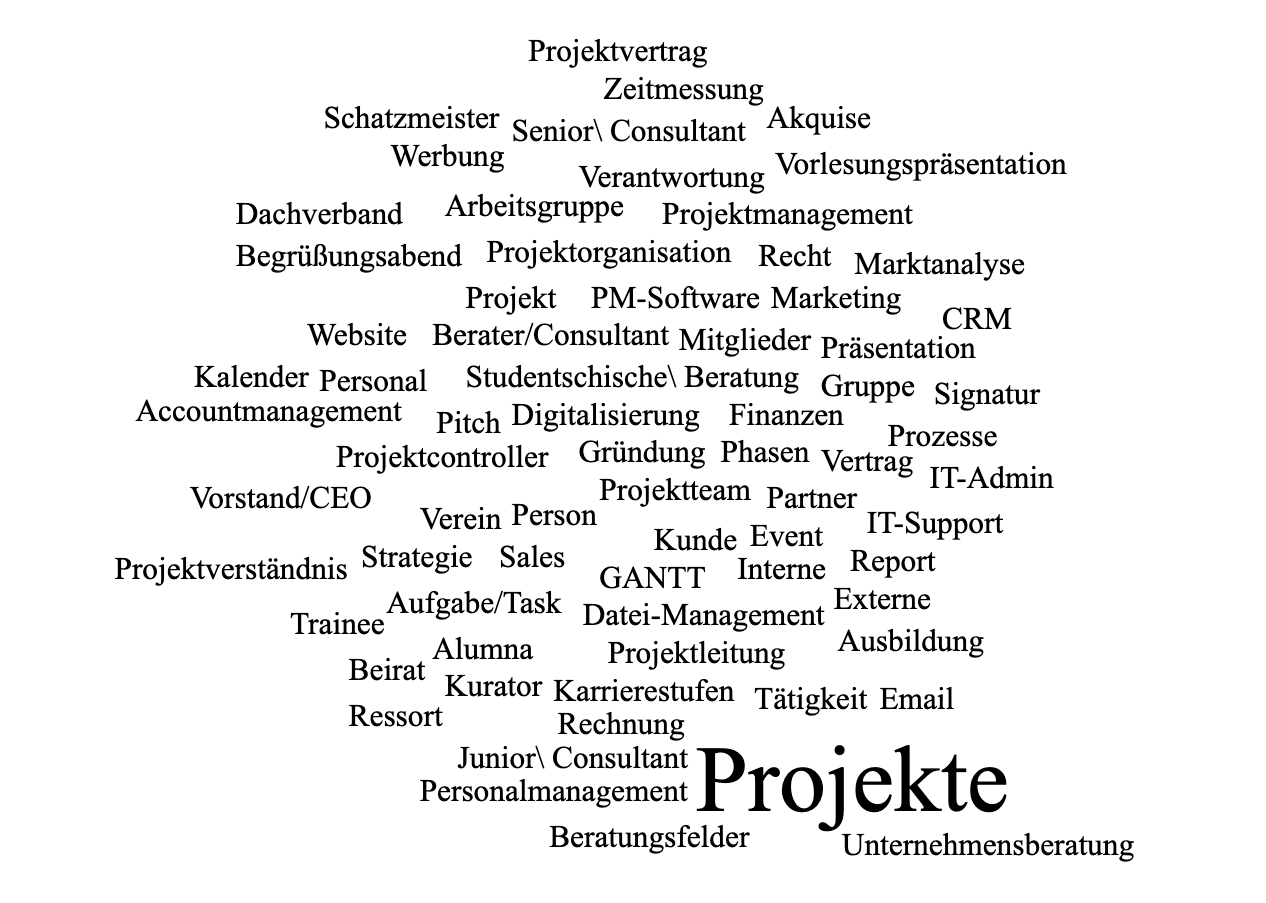
\includegraphics[width=\textwidth]{Images/word-cloud.png}
\end{figure}
\clearpage

\section{Word Graph}
\label{word-graph}
See \autoref{analysis}.
\begin{figure}[h!]
	\centering
	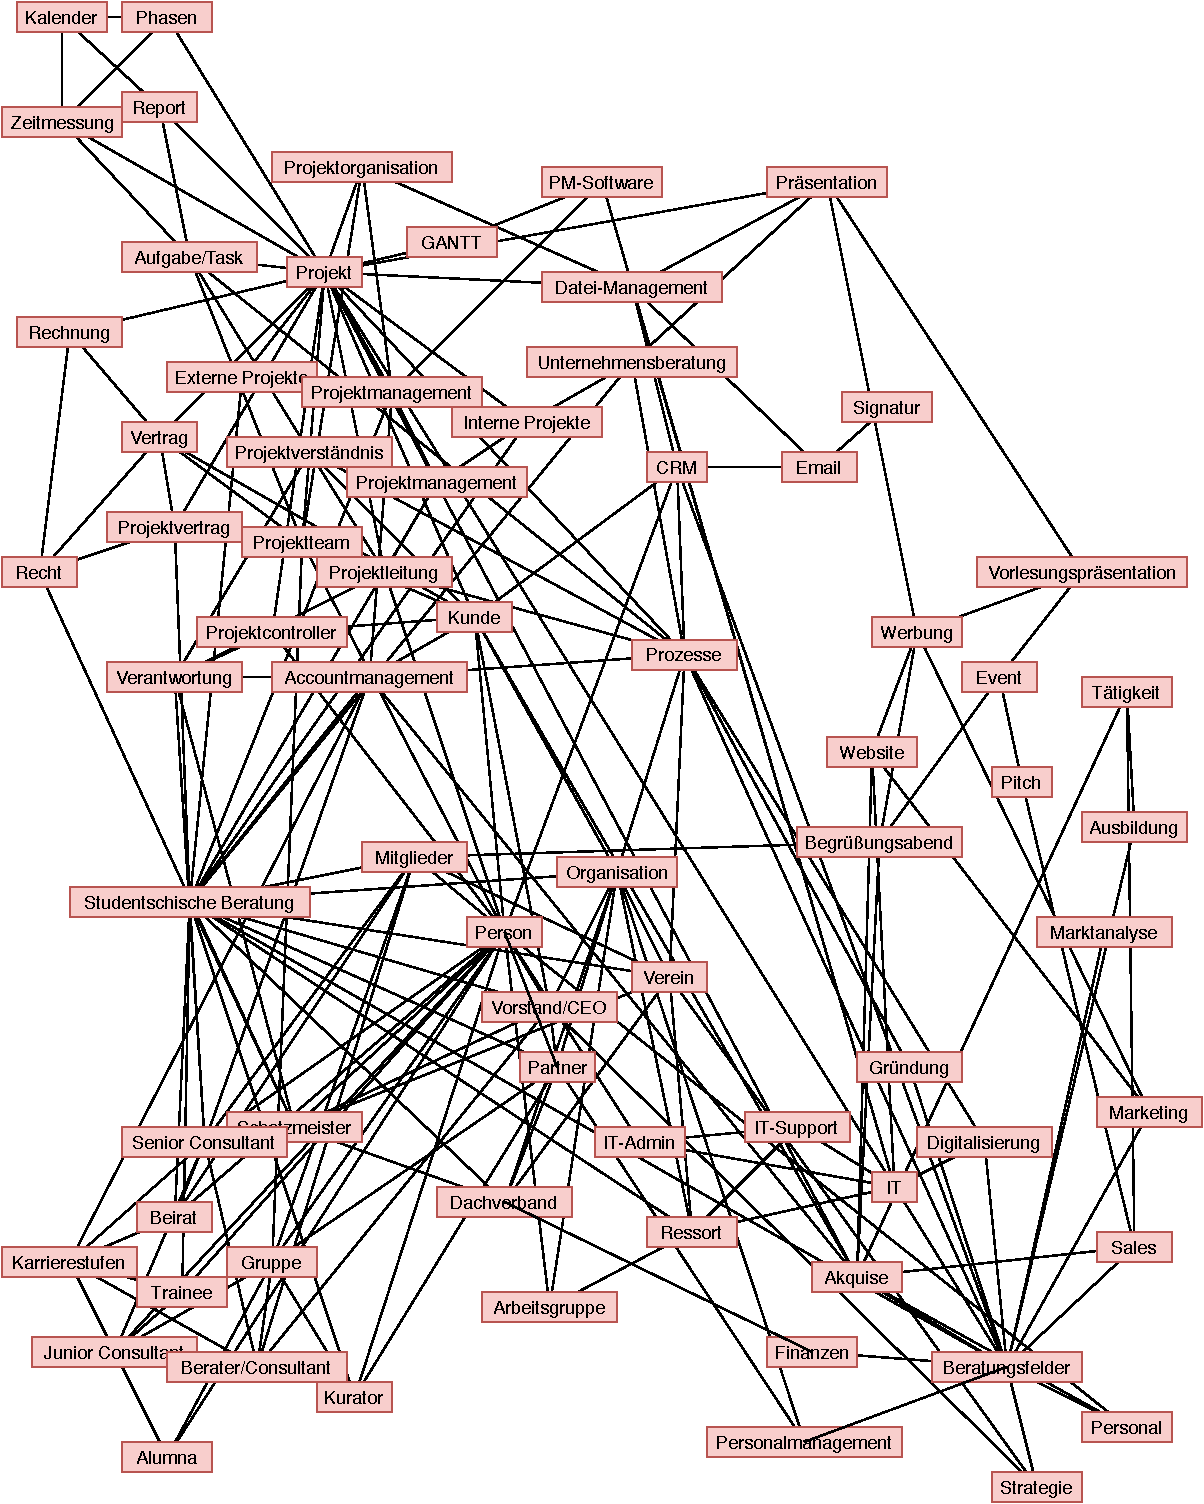
\includegraphics[height=0.9\textheight, width=1\textwidth]{Diagrams/word-graph.pdf}
\end{figure}
\clearpage

\section{Diagrams}
\subsection{General Diagrams}
\begin{figure}[h]
	\caption{Ranks}
	\centering
	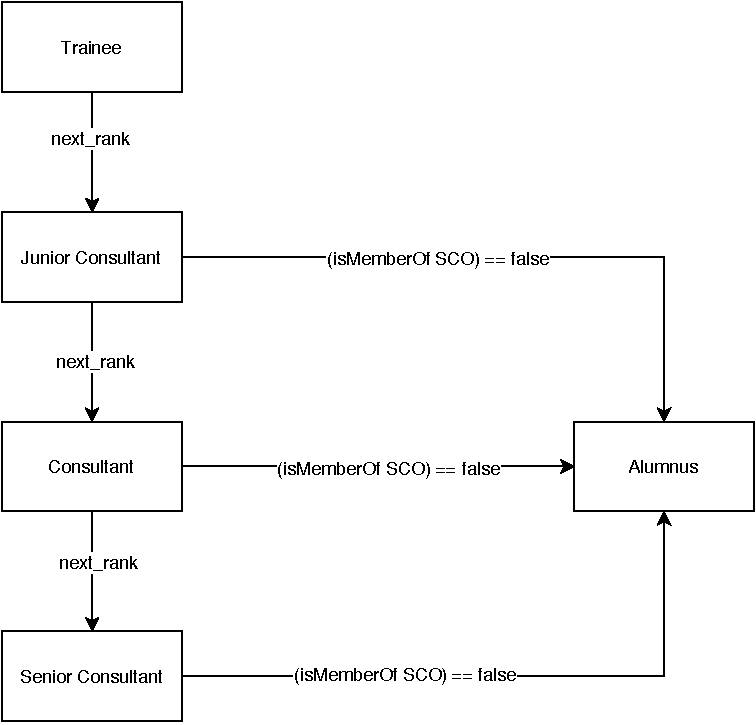
\includegraphics[width=\textwidth]{Diagrams/ranks.pdf}
\end{figure}

\begin{figure}[h]
	\caption{Corporate Officers}
	\centering
	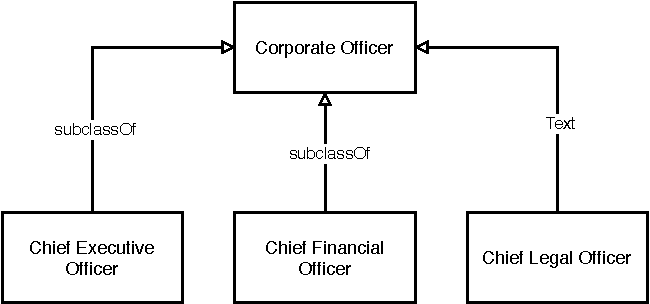
\includegraphics[width=\textwidth]{Diagrams/corporate-officers.pdf}
\end{figure}

\begin{figure}[h]
	\caption{Project Context}
	\centering
	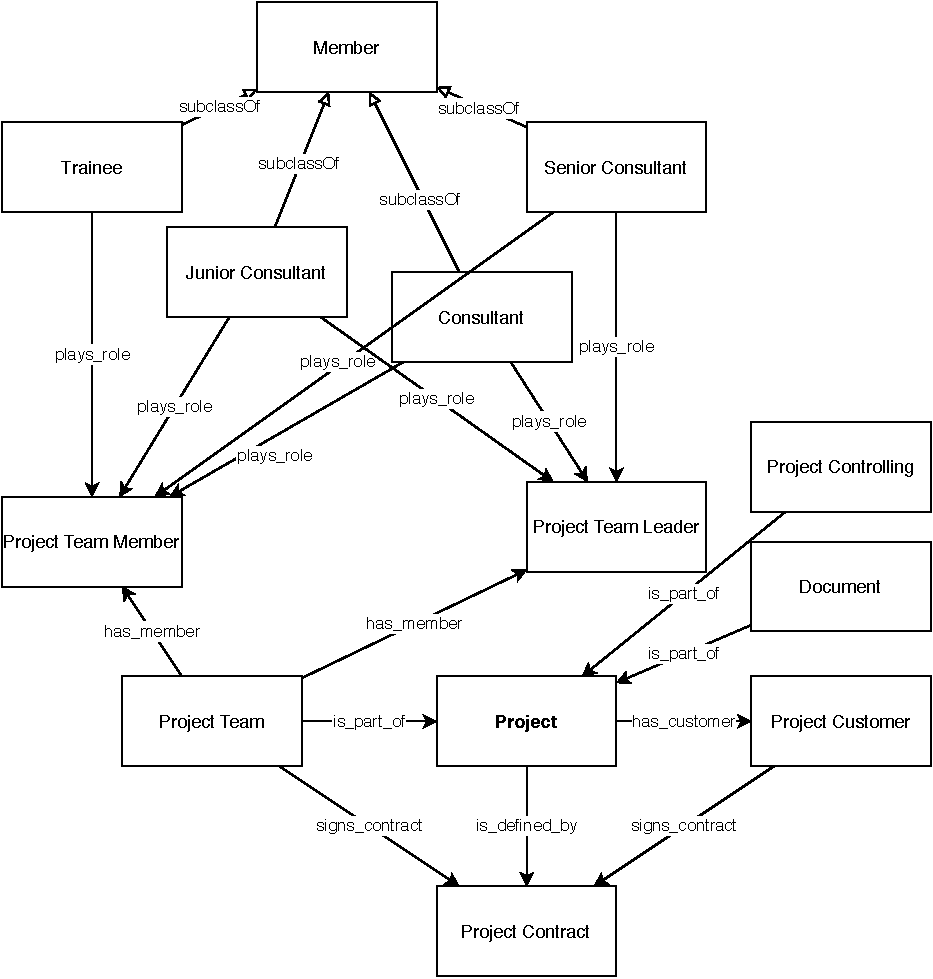
\includegraphics[width=\textwidth]{Diagrams/project-context.pdf}
\end{figure}
\clearpage

\subsection{Process Diagrams}
\label{process-diagrams}
\begin{figure}[h]
	\caption{Project Process}
	\centering
	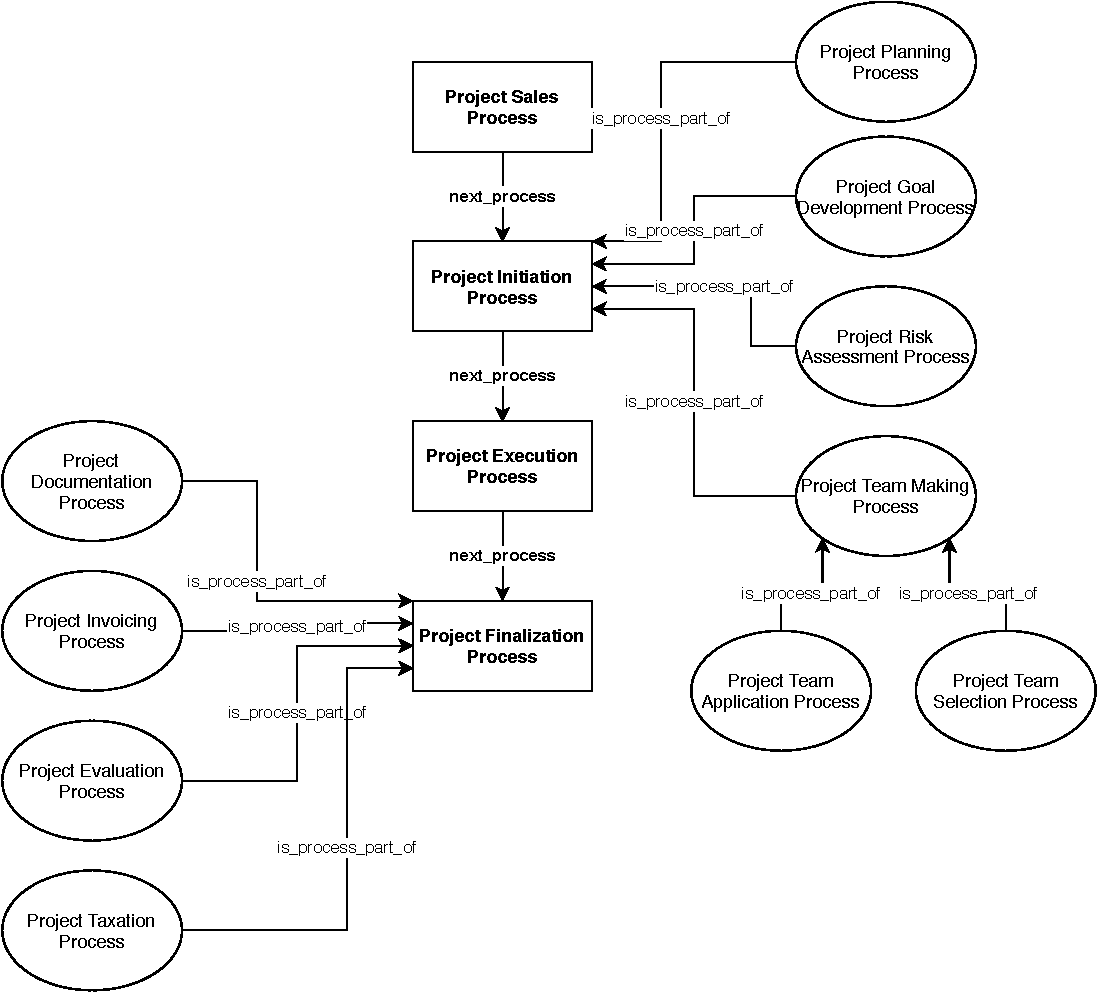
\includegraphics[width=1\textwidth]{Diagrams/project-process.pdf}
\end{figure}

\begin{figure}[h]
	\caption{Human Resources Process}
	\centering
	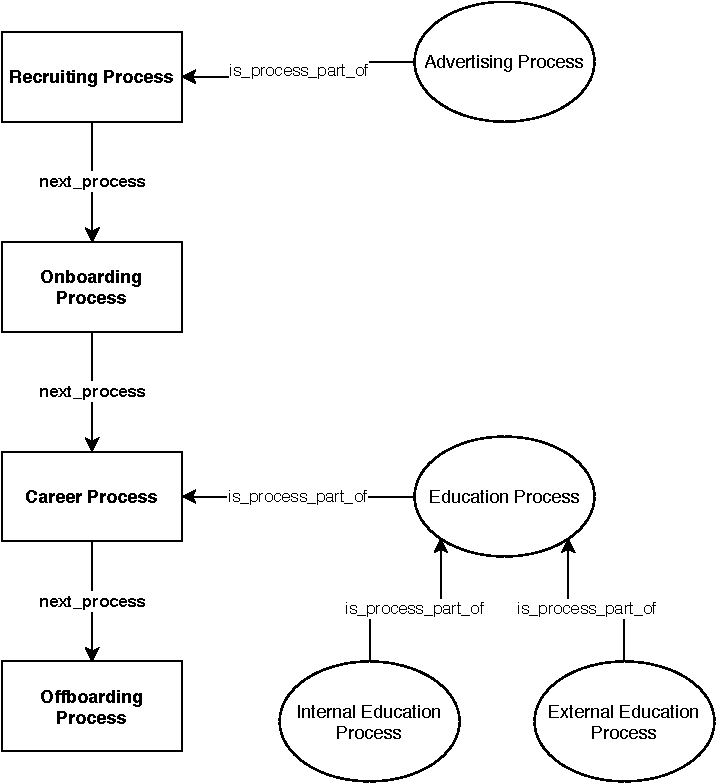
\includegraphics[width=1\textwidth]{Diagrams/hr-process.pdf}
\end{figure}
\clearpage

\section{Dictionary Definitions}
\label{dictionary}
\begin{mdframed}[style=dictionary, frametitle={context {\scriptsize\normalfont\textsc{noun \hfill Merriam-Webster}}}]{
	\small con·​text \textit{\textcolor{teal}{plural}} contexts
		\begin{compactenum}
			\item the parts of a discourse that surround a word or passage and can throw light on its meaning
			\item the interrelated conditions in which something exists or occurs : ENVIRONMENT, SETTING \\
			\textcolor{gray}{\textit{\enquote{the historical context of the war}}}
		\end{compactenum}
	}
\end{mdframed}

\begin{mdframed}[style=dictionary, frametitle={domain {\scriptsize\normalfont\textsc{noun \hfill Merriam-Webster}}}]
	{\small do·​main \textit{\textcolor{teal}{plural}} domains
			\begin{compactenum}
				\item law
				\begin{compactenum}
					\item complete and absolute (see absolute sense 3) ownership of land \\
					\textcolor{gray}{\enquote{\textit{our highways and roads have been in the domain of state and local governments— T. H. White b. 1915}}} \\
					 — compare EMINENT DOMAIN
					\item land so owned
				\end{compactenum}
				\item a territory over which dominion (see DOMINION sense 2) is exercised \\
				\textcolor{gray}{\enquote{\textit{The forest is part of the king's domain.}}}
				\item a region distinctively marked by some physical feature \\
				\textcolor{gray}{\enquote{\textit{a domain of rushing streams, tall trees, and lakes}}}
				\item a sphere (see SPHERE sense 4b) of knowledge, influence, or activity \\
				\textcolor{gray}{\textit{\enquote{the domain of biblical scholarship}, \enquote{outside the domain of city police}}}
				\item mathematics : the set of elements (see ELEMENT sense 2b(3)) to which a mathematical or logical variable is limited \\
				specifically : the set on which a function (see FUNCTION entry 1 sense 5a) is defined
				\item physics : any of the small randomly oriented regions of uniform magnetization in a ferromagnetic substance
				\item mathematics : INTEGRAL DOMAIN
				\item biology : the highest taxonomic category in biological classification ranking above the kingdom (see KINGDOM sense 4b)
				\item biochemistry : any of the three-dimensional subunits of a protein that are formed by the folding of its linear peptide chain and that together make up its tertiary (see TERTIARY entry 1 sense 3c) structure
				\item computers : a subdivision of the Internet consisting of computers or sites usually with a common purpose (such as providing commercial information) and denoted in Internet addresses by a unique abbreviation (such as com for commercial sites or gov for government sites) \\
				\textcolor{gray}{\textit{\enquote{The domain ca is used for sites located in Canada.}}} \\
				also : DOMAIN NAME \\
				\textcolor{gray}{\textit{\enquote{Our domain is Merriam-Webster.com.}}}
		\end{compactenum}
	}
\end{mdframed}

\begin{mdframed}[style=dictionary, frametitle={vocabulary {\scriptsize\normalfont\textsc{noun \hfill Merriam-Webster}}}]
	
	{\small vo·​cab·​u·​lary \textit{\textcolor{teal}{plural}} vocabularies
		\begin{compactenum}
			\item a list or collection of words or of words and phrases usually alphabetically arranged and explained or defined : LEXICON \\
			\textcolor{gray}{\enquote{\textit{The vocabulary for the week is posted online every Monday.}}}
			\item
			\begin{compactenum}
				\item a sum or stock of words employed by a language, group, individual, or work or in a field of knowledge \\
				\textcolor{gray}{\textit{\enquote{a child with a large vocabulary}}, \enquote{the vocabulary of physicians}, \enquote{a writer known for employing a rich vocabulary}}
				\item a list or collection of terms or codes available for use (as in an indexing system) \\
				\textcolor{gray}{\enquote{\textit{… the oldest Sumerian cuneiform writing could not render normal prose but was a mere telegraphic shorthand, whose vocabulary was restricted to names, numerals, units of measure, words for objects counted, and a few adjectives.}} --- \textsc{Jared Diamon}}
			\end{compactenum}
			\item a supply of expressive techniques or devices (as of an art form) \\
			\textcolor{gray}{\textit{\enquote{an impressive musical vocabulary}}}
		\end{compactenum}
	}
\end{mdframed}

\section{Ontology Import Links}
This work lists different ontologies in the related work section. To import them into the Protégé editor, the following links can be used:

\begin{asparadesc}
	\item [\gls{bfo}:] \url{http://purl.obolibrary.org/obo/bfo/2.0/bfo.owl}
	\item [\gls{bpmn}:] \url{https://dkm-static.fbk.eu/resources/ontologies/BPMN/BPMN_2.0_ontology.owl}
	\item [\gls{doap}:] \url{http://usefulinc.com/ns/doap}
	\item [\gls{fibo}:] \url{https://spec.edmcouncil.org/fibo/ontology/master/2019Q4.1/LoadFIBOProd.rdf}
	\item [\gls{foaf}:] \url{http://xmlns.com/foaf/spec/index.rdf}
	\item [\gls{gfo}:] \url{http://www.onto-med.de/ontologies/gfo-basic.owl}
	\item [\gls{gist}:] \url{https://ontologies.semanticarts.com/o/gistCore9.0.0.owl}
	\item [\gls{schema}:] \url{http://schema.org/version/latest/schema.rdf}
\end{asparadesc}

\section{Acknowledgments}
This work was conducted using the Protégé resource, which is supported by grant GM10331601 from the National Institute of General Medical Sciences of the United States National Institutes of Health.

\clearpage
\begin{multicols}{2}
	\printnoidxglossaries
\end{multicols}

\end{document}
